\documentclass[10pt,a4paper]{article}

% images
\usepackage[margin=1.25in]{geometry}
\usepackage{graphicx}
\usepackage{subfig}

\graphicspath{{./figs/}}

\usepackage[title]{appendix}
\usepackage{pgfgantt}

% reference items
\usepackage{enumitem}

\usepackage{lipsum}

\usepackage{setspace}

% links
\usepackage{url}
\usepackage{hyperref}

\usepackage{pdfpages}
\usepackage{pgfplots}

\usepackage{footnote}

% maths
\usepackage{amsmath}
\usepackage{amssymb}
\usepackage{dsfont}
\usepackage{bm}

\usepackage{amsthm}

\theoremstyle{plain}
\newtheorem{theorem}{Theorem}[section]
\newtheorem{claim}[theorem]{Claim}
\newtheorem{lemma}[theorem]{Lemma}

\theoremstyle{definition}
\newtheorem{definition}[theorem]{Definition}

\newenvironment{subproof}[1][\proofname]{%
  \renewcommand{\qedsymbol}{$\blacksquare$}%
  \begin{proof}[#1]%
}{%
  \end{proof}%
}

\newtheorem*{claim*}{Claim}
\newtheorem*{corollary}{Corollary}
\newtheorem*{remark}{Remark}
\newtheorem*{fact}{Fact}

\DeclareMathOperator*{\argmax}{arg\,max}
\DeclareMathOperator*{\argmin}{arg\,min}
 
\usepackage{float}
\usepackage{listings}

\lstset{
    basicstyle=\ttfamily\footnotesize,
    showlines=false,
    breakatwhitespace=false,         
    breaklines=false,                 
    captionpos=b,                    
    keepspaces=false,                 
    numbersep=5pt,                  
    showspaces=false,              
    showstringspaces=false,
	language=Lisp,
	%float, floatplacement=H,
	frame=single,
	breaklines,
	tabsize=4
}

\newcommand{\code}[1]{\texttt{#1}}
\newcommand*\conj[1]{\overline{#1}}
\newcommand*\vect[1]{\bm{#1}}

\bibliographystyle{siam}

\onehalfspacing

\begin{document}

\begin{titlepage}
    \begin{center}

        \vspace*{2cm}
        \includegraphics[width=.25\textwidth]{crest.png}

        \vspace*{1cm}
		{\Large \textsc{A Decentralised Peer-Prediction Market}} \\
		{\textsc{CS907 Dissertation Project - Final Report}}

        \vspace*{1cm}
        \textbf{Thomas Archbold} \\
		1602581 \\~\\
        Department of Computer Science \\
        University of Warwick \\~\\

		September 10, 2020

		\vspace*{1cm}

		Supervised by Professor Matthias Englert

        \vfill

    \end{center}
\end{titlepage}

% Marking Criteria:
% Technical content
% - well read and knowledgeable in the project's subject
% 	area;
% - good insight into the project's specific topic; 
% - effective analysis of the problems and issues relating to the project's
%   aims;
% - quality of design work and appropriate choice of methods and tools;
% - effective testing/validation regime;
% - quality of results and analysis; 
% - critical evaluation of the project;
% - quality of practical/technical work and overall level of technical
%   achievement
% 
% Project management and organisation
% - consistent progress;
% - initially unforeseen problems well detected and overcome; 
% - necessary research, analysis and design work completed;
% - completeness of project overall
%
% Communication skills
% - clear exposition of the aims, achievements and limitations of the %
%   project;
% - coherence, structure and composition of report;
% - software and hardware appropriate documented;
% - readability and appropriate length

% Structure
% - Introduction
% - Literature Review/Background Context
% - Motivation and Statement of Goals
% - Design overview
% - Implementation details
% - Project Management
% - Evaluation

\input{sections/abstract}

\pagebreak
\tableofcontents

\listoffigures
\lstlistoflistings

\pagebreak

\section{Introduction}

\label{sec:introduction}

Prediction markets are exchange-traded markets\footnote{Markets in which all
transactions are routed through a central source.} which allow users to trade
on the outcomes of future events as opposed to traditional financial
instruments. Users participate by placing bets and buying or selling shares in
the markets these bets give rise to. Since users stake their own money, market
prices should indicate the true beliefs of the userbase and the perceived
likelihood the events have of occurring. Different users will have different
beliefs and knowledge informing their decisions, hence prediction markets provide
a means of aggregating information on events of interest using ``the wisdom of
the crowd''. Shares in these markets are usually traded between \$0 and \$1,
and for binary events a market will typically pay out \$1 for every share held
for a positive outcome, and \$0 otherwise.

Traditional prediction markets are centralised in the sense that the system
provides the possible bets on which to trade, and traders simply choose the
price point and stake at which to participate. Since the system knows all
possible bets beforehand it is simple for it to determine the outcomes of the
markets and pay out the winnings accordingly. There are two issues with this
centralised approach: firstly, it restricts the types of bets that can be made,
since they must be explicitly offered by the market maker; secondly, it
operates on trust -- there is nothing to stop the central market maker from
manipulating the system for their own gain. We aim for a system that avoids
both of these issues.

In this project we implement a \emph{decentralised} prediction market in which
the userbase itself defines the markets and determines their outcomes -- these
are decided by consensus among groups of users, known as arbiters. This removes
the need for a trusted centre, however with no central moderator bets may
become ambiguous or their outcomes subjective, and arbiters may still attempt
to manipulate the outcome of the market for their own gain by submitting false
reports. It is also important that users continue to act according to their
true beliefs, so that we may gather useful information on the events. We base
our design on the incentive compatible peer prediction mechanism introduced by
Freeman, Lahaie, and Pennock~\cite{Freeman2017}, which allows us to crowdsource
market outcomes while incentivising users to act truthfully in all stages of
the prediction market.

The rest of this dissertation is structured as follows: in
Section~\ref{sec:background} we introduce the various types of prediction
markets and different approaches to their implementation. In
Section~\ref{sec:literatureReview} we give an overview of existing markets and
the current literature within the algorithmic game theory community. In
Section~\ref{sec:goals} we state our goals for the project and justify our
reasons for undertaking it. Section~\ref{sec:design} covers the high-level
design of the market on which we base our implementation and introduces some
theoretical considerations we take into account. In
Section~\ref{sec:implementation} we discuss the details of our implementation
of the decentralised market, including the tools we use to develop it.
Section~\ref{sec:projectManagement} covers our approach towards project
management. Finally, in Section~\ref{sec:evaluation} we reflect on the
project's successes and suggest areas for improvement.

\section{Background}

\label{sec:background}

\subsection{The Information Aggregation Problem}

Consider the following problem within algorithmic mechanism design known as the
\emph{information aggregation problem}~\cite[Ch.~26]{AGTBook}. An individual
known as the ``aggregator'' wishes to obtain a prediction about an uncertain
variable which will be realised at some point in the future. There are a number
of individuals known as the ``informants'' who each hold sets of information
about the variable's outcome. The goal is to design a mechanism that extracts
the relevant information from the informants and uses it to provide a
prediction of the variable's realisation. In an ideal setting the mechanism
should produce the same prediction as an omniscient forecast that has access to
all information available to all informants. This may not be viable in
practice, since each agent's information is private, and so the mechanism must
incentivise them to act in the desired truth-telling manner.

A prediction market is one mechanism that can provide such a forecast. In this
setting the aggregator creates a financial security whose payoff is tied to the
outcome of the variable. In the simpler case of binary events, such a security
may pay out \$1 for each share held if the variable has a ``true'' or ``yes''
outcome, and \$0 otherwise, however other types of markets can be created,
including discrete (``will the result of the match be a home win, away win, or
a draw?''), continuous (``what will be the highest measured temperature in
Coventry in September?''), or any combination of these types. Informants are
then able to participate in the market induced by the security by trading
shares according to their beliefs: those who believe, for example, that global
warming is real might buy shares at a given price in the market, ``the global
average temperature in 2020 will be higher than that in 2019'', while deniers
may be inclined to sell shares. The share price will be adjusted accordingly,
and the aggregator can view the current price as the informant's combined
belief of the outcome of the event.

In the \emph{partition model of knowledge} there is a set $\Omega$ of possible
states of the world and at any moment the world is in exactly one state $\omega
\in \Omega$, though the informants do not know which. Each informant $i$ may,
however, possess partial information regarding this true state, represented by
a partition $\pi_i$ of $\Omega$. The agent knows in which subset of this
partition the true world state lies, but does not know the exact member of
which is true. Given $n$ agents, their combined information $\hat{\pi}$ is the
coarsest common refinement of the partitions $\pi_1, \ldots, \pi_n$.\footnote{A
partition $\alpha$ of a set $X$ is a refinement of a partition $\rho$ of $X$ if
every element of $\alpha$ is a subset of some element of $\rho$. In this case
$\alpha$ is \emph{finer} than $\rho$ and $\rho$ is \emph{coarser} than
$\alpha$.}

We also assume a common prior probability distribution $P \in \Delta^{\Omega}$
which describes the probabilities that all agents assign to the different world
states before receiving any information. Once each agent receives their partial
information, they form their posterior beliefs by restricting the common prior
to the subset of their partition in which they know the true state to lie.  A
\emph{forecast} is an estimate of the expected value of the function $f :
\Omega \rightarrow \{0,1\}$, known as an \emph{event}, which equals one for
exactly one subset of $\Omega$ and 0 otherwise.

As mentioned, there is an ideal ``omniscient'' forecast that uses the
distribution $P$ restricted to the subset of $\hat{\pi}$ in which the true
world state lies -- this is difficult to achieve given the private nature of
each agent's information. The goal is therefore to design a mechanism to
incentivise agents to reveal their private information such that in equilibrium
we achieve a forecast as close as possible to the omniscient one. Prediction
markets offer the agents the chance of financial gain for revealing information
on the expected value of $f(\omega)$, and the share price of the security can
be interpreted as the collective forecast of the agents. In the remainder of
the section we shall outline some of the different approaches to designing the
market mechanism: the best choice will vary for the setting and will depend on
what is tractable given the types of bets that are on offer. First we shall
introduce combinatorial markets.

\subsection{Combinatorial Prediction Markets}

A \emph{combinatorial} prediction market is one in which the total state space
$\Omega$ is the product space of a collection of base events. Suppose knowing
the outcome of a given event cannot be predicted with certainty even if the
outcomes to all other base events are known, and we wish to provide the
opportunity to trade on any outcome $\omega \in \Omega$: with a set of base
events of size $\mathcal{|E|}$ we would have a total outcome space of size
$2^\mathcal{|E|}$.  With such a large outcome space it may therefore be
impossible to even all list the securities available in such a market.
Combinatorial markets can make use of ``expressive'' bidding languages that
represent collections of securities succinctly, including \emph{combined
orders} and \emph{compound orders}.

Combined orders allow a user to trade a collection of securities by specifying
the securities they wish to buy or sell together as a bundle along with limit
prices for each constituent security. If there is even a single security in the
bundle that is not at least as ``good''\footnote{If we are buying we want a
price less than or equal to the limit price, while the opposite is true if we
are selling.} as its limit price, then no trade is made. If an agent were to
trade on these securities in a non-combinatorial market, they would need a
trade to be executed on each one individually. Throughout the execution of such
a sequence of trades, however, market prices would be subject to change, and in
the worst case these fluctuations could reduce or even reverse the utility of
participating in such trades. Combined orders therefore protect its
participants from such risk. Calculating the assignment of securities to buyers
in such a setting is as hard as the winner-determination problem faced by a
combinatorial \emph{auction}, which known to be NP-hard.

Compound orders are generalisations of combined orders and allow users to trade
on any Boolean expression on the set of base events. Now again the size of the
outcome space is $2^\mathcal{|E|}$, but now there are $2^{2^\mathcal{|E|}}$
subsets of these outcomes expressible with Boolean formulae. Agents now place
orders by requesting $q$ shares of the security $S_{\phi|\psi}$ at share price
$p$, where $S_{\phi|\psi}$ pays out \$1 if both Boolean formulae $\phi$ and
$\psi$ are true, \$0 if only $\psi$ is true, and refunds the user if $\psi$ is
false. These orders will yield a payoff $\gamma^{\langle \omega \rangle}$
depending on the state $\omega \in \Omega$, and can be written as:
%
\[
	\gamma^{\langle \omega \rangle} = q \cdot \mathds{1}_{\omega \in \psi}
	(\mathds{1}_{\omega \in \phi} - p)
\]
%
in which $\omega \in \phi$ means outcome $\omega$ satisfies the Boolean formula
$\phi$. This says that the order will receive an overall payoff of zero if the
true world state $\omega$ does satisfy $\psi$, meaning the order is invalid and
refunded to the user. Otherwise, the user will receive a payout of $(1-p)$ for
each share they bought if $\omega$ satisfies $\phi$. If the event does not
occur they will lose what they paid and receive a payoff of $-p$ for each of
$q$ shares. Each user $i$ has a payoff vector $\gamma_i$ induced by submitting
orders. It is the job of the auctioneer to determine which orders to accept.
Let $\alpha_i \in \{0,1\}$ indicate whether the auctioneer accepts an order
from user $i$. Since they will collect the money paid by the trader and payout
their winnings according to each user's payoff vector, the auctioneer receives
payoff:
%
\[
	\gamma_a = \sum_i -\alpha_i \gamma_i
\]
%
The \emph{indivisible matching problem} asks that, given a set of orders, does
there exist a set of $\alpha_i \in \{0,1\}$ and $\sum_i \alpha_i \ge 1$ such
that for any outcome $\omega$ the auctioneer receives payoff $\gamma_a^{\langle
\omega \rangle} \ge 0$? In other words, the auctioneer is looking to accept
some bundle of orders \emph{without risk}.

\textbf{Example} Suppose $\mathcal{E} = \{X_1, X_2\}$ and there are two orders:
agent 1 wishes to buy two shares of security $S_{X_1}$ at \$0.6 per share while
agent 2 wishes to sell one share of security $S_{X_1,X_2}$ for \$0.2 per
share. Assuming the auctioneer accepts both orders, the payoffs are as follows
(note player 2's payoff vector is negated since they are selling):
%
\begin{equation*}
	\begin{aligned}
		\gamma_1 & = \left\langle \begin{matrix}
			\gamma_1^{X_1,X_2} &
			\gamma_1^{X_1,\bar{X_2}} &
			\gamma_1^{\bar{X_1},X_2} &
		\gamma_1^{\bar{X_1},\bar{X_2}} \end{matrix} \right\rangle 
%
		 = \left\langle \begin{matrix}
			2(1-0.6) & 2(1-0.6) & 2(-0.6) & 2(-0.6) \end{matrix} \right\rangle \\
%
		\gamma_2 & = - \left\langle \begin{matrix}
			1(1-0.2) & 1(-0.2) & 1(-0.2) & 1(-0.2) \end{matrix} \right\rangle \\
%
		\gamma_a & = \left\langle \begin{matrix}
			0 & -1 & 1 & 1 \end{matrix} \right\rangle
	\end{aligned}
\end{equation*}
%
Accepting both orders is therefore not a valid solution to the indivisible
matching problem since in the event that $\omega = \{X_1,\bar{X_2}\}$ the
auctioneer would have to run a loss. In fact, finding a solution to the
indivisible matching problem is NP-complete~\cite[Ch.~26]{AGTBook}. Although we
do not focus on combinatorial prediction markets in this project, it is useful
to illustrate the challenges of designing efficient market mechanisms. In
particular, we are concerned with low liquidity, which arises when there is too
little participation in the market for a trade to be executed.

\subsection{Trading Mechanisms}

\label{sec:tradingMechanisms}

\subsubsection{Continuous Double Auctions}

Trading mechanisms are responsible for deciding which trades are executed, in
what quantities, and at which price points. In the previous section, although
users had to submit orders of a particular form, the auctioneer was free to
accept any subset of the orders received: this section expounds upon \emph{how}
trades may be chosen to be executed. These are called market trading
mechanisms, and include double auctions, market call auctions, and automated
market makers. A Continuous Double Auction (CDA) is a mechanism in which buyers
are matched with sellers of a particular security. The market maker keeps an
order book that tracks the bids, submitted by those looking to buy, and the
asks, submitted by those looking to sell. Traders arrive asynchronously and
place orders, and when two opposite orders match the trade is executed. CDAs
are traditionally used in highly liquid markets, such as the New York Stock
Exchange, where there are many bids for a given ask and vice versa. An issue
with this approach is that it relies on there always being a willing buyer and
seller at a particular price and quantity in order to execute a trade.
Prediction markets have far fewer participants than stock exchanges, and the
problem of low liquidity is made even worse in combinatorial markets, in which
a trader's attention is split among an exponential number of securities. This
makes the likelihood that a buyer and seller are looking to trade on the same
event exceptionally small. Prices may also not be informative of the true
beliefs held by traders in CDAs: since all traders can see bids and asks as
they are submitted sellers may be encouraged to ask less than what they truly
believe to be a security's ``true'' value in order to undercut another seller
and make a profit. This is not useful in a prediction market setting, where we
want to elicit the true beliefs from users.

These problems arising from market low liquidity can be averted by using an
automated market maker, in which a price maker is nearly always willing to
accept both buy and sell orders at a certain price. Participation in the market
will have an effect on these prices, the exact nature of which will be down to
the market maker. This ensures that, if the price is desirable, participants
are always able to make a trade. An automated market maker is not typically
used in real-world markets since always assuming the opposite side to any trade
would likely result in significant losses for ``the house''; in play-money
markets this is not such an issue as losses are less detrimental and have no
real-world negative value. In general there are three properties that an
automated market maker should satisfy in order to be of practical use: traders
should have an incentive to participate in the market whenever their beliefs
would change the price; the computation of market prices should be tractable;
and the market's loss should be bounded. We present two options for
implementing automated market makers: as a parimutuel market or using a Market
Scoring Rule.

\subsubsection{Parimutuel Markets}

In parimutuel markets traders wager money their choice of outcomes from a
mutually exclusive and exhaustive set. When the event's outcome is realised the
total wagered money is split between those who wagered correctly, in proportion
to the size of their bet. In order to accommodate traders selling shares prior
to the outcome of the event, \emph{dynamic} parimutuel markets incorporate a
cost function that varies the price of a single share due to trading activity.
An example of one such cost function is the share-ratio cost function. Suppose
we have an outcome space $\Omega$ and let $q_j$ denote the total number of
shares for event $j \in \Omega$. Let $\vect{q} = (q_1, \ldots, q_{|\Omega|})$
be the vector of outstanding shares of all contracts. The share-ratio cost
function is:
%
\[
	C(\vect{q}) = \sqrt{\sum_j q_j^2}
\]
%
A trader wishing to buy $q_j' - q_j$ shares of security $j$, thus changing the
number of outstanding shares of $j$ from $q_j$ to $q_j'$, pays the market
$C(\vect{q}_{-j}, q_j') - C(\vect{q})$.\footnote{We use $\vect{q}_{-j}$ to
denote the vector $(q_1, \ldots, q_{j-1}, q_{j+1}, \ldots, q_{|\Omega|})$.}
There is a corresponding price function $p_j$ that gives the price for
purchasing an infinitesimal quantity of shares in security $j$ and is used to
quote a share price to market participants:
%
\[
	p_j = \frac{q_j}{\sum_k q_k^2}
\]
%
This share price $p_j$ should not be used to calculate the cost of a
transaction since an agent's participation in the market will instantly change
this value. The purpose of a prediction market is to elicit private information
on some future event: we use the information we have on user participation in
the market to compute probability $\pi_j$ of outcome $j$ as $\pi_j = p_j^2$.

\subsubsection{Scoring Rule Markets}

A scoring rule is used to assign probabilities to a set of mutually exclusive
outcomes. When the scoring rule is proper\footnote{A scoring rule giving the
highest expected reward for reporting the true distribution.}, it can be
converted to an automated market maker that uses a Market Scoring Rule
(MSR)~\cite{Hanson2003}.  Again at the heart of a MSR is the cost function
$C(\vect{q})$, which is a means of recording the total amount of money spent in
the market by traders as a function of the total number of shares in
circulation. Traders wishing to purchase $q_j' - q_j$ shares of security $j$
must again pay $C(\vect{q}_{-j}, q_j')-C(\vect{q})$. Note that in both
parimutuel markets and scoring rule markets, these rules also encode sell
transactions, in which case $q_j' < q_j$. We cannot use $C$ directly to quote a
share price to the user since we first need to know what quantity they to buy
or sell: we use its derivative $p = \partial C / \partial q_j$ to again quote
the cost for an infinitesimal quantity of shares.  As an example, the quadratic
scoring rule gives some reward $Q(\vect{r},i)$ if the $i$th event occurs, given
the probability vector $\vect{r}$. The cost function corresponding to the
quadratic scoring rule is:
%
\[
	C(\vect{q}) =
	\frac{\sum_j q_j}{|\Omega|} + \frac{\sum_j q_j^2}{4b}  +
	\frac{\left( \sum_j q_j \right)^2}{4b|\Omega|} - \frac{b}{|\Omega|}
\]
%
Scoring rule markets typically pay out \$1 for each share held of a security
whose outcome was positive, and \$0 otherwise. In contrast, parimutuel markets
can have a different payoff per share since they pay out an equal portion of
the total amount wagered per share held to winning shareholders. This project
implements the former. The following section will outline some existing
prediction markets as well as important results from the literature.

\section{Literature Review}

\label{sec:literatureReview}

% Iowa Electronic Markets
% PredictIt, PredictAlot
% Intrade
% Rational expectations - demand not same as traditional market
% PredictIt disputes: wording

\subsection{The Iowa Electronic Markets}

The Iowa Electronic Markets (IEM) are real-money prediction markets developed
by the University of Iowa~\cite{IEM} that have been running since 1988. They
allow users to buy and sell contracts based on the outcome of U.S. political
elections and economic indicators, and are currently offering markets for the
winning party of the 2020 U.S. presidential election, the vote share between
the Democratic and Republican parties in the 2020 U.S. presidential election,
and the compositions of the houses of Congress, House of Representatives, and
U.S. Senate after the outcome of the 2020 U.S. congressional elections. The
number of markets offered is small and the topics are kept relevant to current
events, meaning there is likely to be high liquidity for any security a user
wishes to trade in. This has allowed the markets to predict the results of
political elections with more accuracy and less error than traditional polls:
for the presidential elections between 1988 and 2000, three-quarters of the
time the IEM's market price on the day each poll was released was more accurate
for predicting vote share than the poll itself~\cite[pg.~19]{WisdomOfCrowds}.
These markets inspired similar markets in the forms of the Hollywood Stock
Exchange, NewsFutures, and the Foresight Exchange report, which achieved
similar successes despite not using real money. 

\subsection{Combinatorial Markets}

An issue with these markets is that they are restrictive in the bets they
offer. Although this can be beneficial in that they provide a focused and
liquid market in which to trade, they are less expressive. A combinatorial
prediction market drastically increases the number of outcomes that can be
predicted by offering securities on propositions that can be combined in
various ways. One example of such a market is
\emph{Predictalot}~\cite{Predictalot}, a combinatorial prediction market
developed by Yahoo! that allowed users to trade securities in the 2010 NCAA
Men's Division I Basketball Tournament. The tournament sees the top 64 teams
play 63 games in a knockout competition, yielding a total outcome space of size
$2^{63}$. \emph{Predictalot} then kept track of the odds, computing them by
scanning through all of the predictions made by users. This application served
as the original inspiration for this project to explore prediction markets.
Using a Market Scoring Rule for such a market would involve computing a
summation over the entire outcome space $\Omega$, an intractable, \#P-hard
problem akin to counting the number of subsets in a list of integers that sum
to zero. Instead, they use importance sampling, a technique for estimating
properties of a particular probability distribution using only samples
generated from a different distribution. This ``naive'' approach is then
improved upon by the work of Dud\'ik, Lahaie, and Pennock~\cite{Dudik2012}, who
use convex optimisation and constraint generation to develop a tractable market
maker. This approach is a compromise between treating all securities as
independent and a fully combinatorial, ``ideal'' market maker, but still allows
for information to be gathered among related securities. This allows for them
to compute odds that make sense: for example, a large bet on a team to win the
entire tournament would also increase their odds at every other stage in the
tournament, since they must win these to even reach the final. Kroer, Dud\'ik,
Lahaie, and Balakrishnan~\cite{Kroer2016} use integer programming to remove
trades which are always profitable and incur no risk. In other words, they
ensure all trades are arbitrage-free. On top of achieving bounded loss, a
crucial element behind a market mechanism operating in the real world and
avoiding bankruptcy, avoiding arbitrage is desirable as it leads to more
accurate forecasts: since users cannot make risk-free profits, they are forced
to bet according to their true beliefs.

\subsection{Decentralised Markets}

All examples so far have involved a centralised market mechanism. These types
of systems involve a central authority providing the securities upon which
users may trade and then verifying their outcome. \emph{Decentralised} markets
allow the users to specify the securities themselves and trade shares in them.
Several examples of decentralised markets exist, and they are often implemented
with cryptocurrencies. Peterson et al.~\cite{Peterson2015} study the setting
and implement the oracle at the heart of \emph{Augur}~\cite{Augur}, a
decentralised prediction market built upon the Ethereum blockchain, which
launched in 2018. It allows users to offer predictions on any topic, and
markets may be either categorical, which are similar to binary markets in which
the winner takes all, or scalar, which offer users a spectrum of outcomes in
which to invest. As in many decentralised markets, outcomes of events are then
resolved by the users, and in \emph{Augur} users are incentivised to report
truthfully by way of paying reporting fees: users back their report by
depositing tokens, and token holders are then entitled to the trading fees
generated.  Although this persuades against manipulation, it has not been shown
whether this system achieves any theoretical guarantees of truthful reporting.

As can often be the case with real-money markets, the platform had quickly
devolved into an assassination market~\cite{AugurDeathMarket} -- originally
this referred to the case where users created markets on the deaths of certain
people, which then incentivised their assassination. A user could stand to
profit by placing a bet on the exact time of their death, and ensure this bet
was profitable by assassinating the subject. More generally this refers to the
users of a prediction market having the ability to influence a market's outcome
and acting on this opportunity. Another issue with \emph{Augur} is the option
to report a market's outcome as ``invalid'': this is for the case where the
user-made bet is too ambiguous to decided, such as, ``Bayern Munich will play
well against Paris Saint Germain''.

Other decentralised markets based on cryptocurrencies exist, including
\emph{Omen}~\cite{Omen} and \emph{Hivemind}~\cite{Hivemind}. The former is
similar to \emph{Augur} in that it allows users to create markets for any bet
they like and whose outcomes are not decided by the system itself. Whereas
\emph{Augur} uses a reputation system whereby users back their report of a
market's outcome with \$REP tokens, \emph{Omen} asks the market creator to
supply an ``oracle'' through which the outcome can be determined. This oracle
can even be \emph{Augur}. Although this may solve the ``invalid'' outcome
option for ambiguous bets, it may introduce bias into the process of outcome
determination. For example, suppose a user creates a market for ``The
Democratic nominee will tell a lie during tonight's debate'' and lists the
oracle as the conservative news channel, Fox News. Users would then trade on
how they think the oracle will report the outcome, and not what they believe
the outcome will be themselves. An important aspect of decentralised markets
must therefore be that the outcome is determined by the community, not a single
source. 

In contrast to \emph{Augur}, which implements a traditional order book using
Ethereum, \emph{Omen} uses an automated market maker to provide liquidity to
its securities. As we have discussed, automated market makers can be
implemented via Market Scoring Rules. Hanson~\cite{Hanson2003} shows that we
can use any strictly proper scoring rule to implement an automated market
maker: with such scoring rules, agents maximise their expected utility by
truthfully revealing their predictions. In particular, in this project we
implement the peer prediction market introduced by Freeman, Lahaie, and
Pennock~\cite{Freeman2017}, which specifies a mechanism to trade bets and
crowdsource outcome determination. Market outcomes are decided by asking users
for reports, similarly to \emph{Augur}. All they require is that the rule is
strictly proper, giving plenty of choice to study the effects different rules
have on user and price behaviour. While the choice of scoring rule is less
important than the mechanism by which market outcomes are determined, a recent
work by Liu, Wang, and Chen~\cite{Liu2020} introduces scoring rules for the
setting where the aggregator has access only to user reports, which they call
Surrogate Scoring Rules (SSRs). This appears to be an interesting avenue to
further explore and adapt to a prediction market. One assumption they make,
however, seems incompatible with the decentralised setting in that they require
all events to be independent.  Given that users can create a market for
\emph{any} bet, this condition is impossible to ensure. Since SSRs can be
strictly proper under certain conditions, they may be suitable as the Market
Scoring Rule in \cite{Freeman2017}. 

Other prediction markets existed in \emph{PredictIt}~\cite{PredictIt} and
\emph{InTrade}~\cite{InTrade}, both offering markets for various political and
economic events. However, both experienced disputes largely related to the
wording of the available to trade and the ambiguity in their resolution. For
example, a bet offered on \emph{PredictIt} was, ``Who will be Senate-confirmed
Secretary of State on March 31, 2018?'', and although Rex Tillerson was fired
in the middle of March, he was officially the secretary of state until midnight
of the 31st, leading to confusion among users in what they are trading on and
therefore inaccuracies in the predictions it elicited. This will be a problem
inherent to any prediction market that allows users to specify their own bets,
and while the work of Freeman et al.~\cite{Freeman2017} mitigates the problem of
determining the outcome by setting it to the proportion of users reporting a
``yes'' outcome, this does nothing to penalise the initial creator for
introducing an ambiguous market.

\begin{figure}[h]
	\centering
	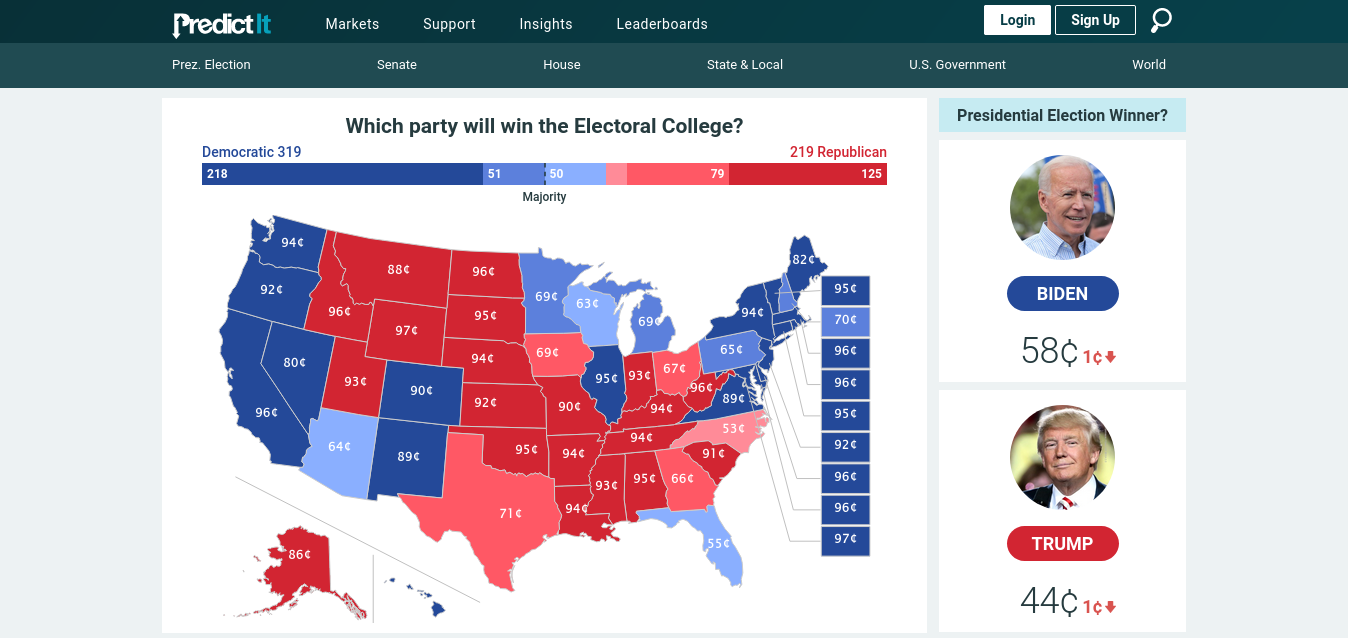
\includegraphics[width=\textwidth]{predictit}
	\caption{The \emph{PredictIt} prediction market for the 2020 U.S.
	presidential election. As of \today\ Joe Biden is perceived to be more
	likely to become President.}
	\label{fig:predictit}
\end{figure}

\subsection{A Note on \emph{Predictalot}}

As we will cover in the following section, the goals of this project are more
concerned with the game-theoretic aspects of implementing a decentralised
prediction market. This involves encouraging users to act in the desired
manner, which in our case means ``telling the truth'' about both their beliefs
on an event's outcome and their observation of the result. Since combinatorial
prediction markets are often centralised, meaning bets come straight from the
system and not its users, all users have to do is choose to participate in the
market at what they view as the correct price, hence there is much less
opportunity for manipulation. For this reason, combinatorial prediction markets
are more concerned with the computational aspects of offering combinatorial
securities to its traders, and in particular how to compute accurate prices on
combinations of interrelated securities. Both decentralised and combinatorial
settings are interesting in their own right, and both can achieve an added
level of expressiveness compared to a traditional prediction market such as the
IEM. Here we will briefly describe approaches taken to improving the efficiency
of pricing in the \emph{Predictalot} prediction market.

We will first discuss the hardness of using a Market Scoring Rule to calculate
prices in a combinatorial market. The class NP is the set of decision problems
for which, given an input to the problem and a proposed solution, the
``certificate'', verification that the certificate is indeed a correct solution
can be done in polynomial time. By self-reducibility, the search version of the
problem is no harder than the decision version. The class \#P consists of
\emph{functions} that count the number of solutions to NP search problems. A
function $g$ is \#P-hard if, for every function $f$ in \#P, given an oracle for
$g$ we can compute $f$ in polynomial time -- that is, computing $g$ is at least
as hard as any other function $f$ in \#P. Chen et al.~\cite{Chen2008} show that
computing the price and cost functions of a MSR in a combinatorial market is
\#P-hard, even when traders are restricted to betting on the disjunctions or
conjunctions of two events. They do this via a reduction to the \#P-hard
function \textsc{\#2-SAT}, which counts the number of satisfying assignments of
a CNF formula, where each clause has two literals. 

Dud\'ik et al.~\cite{Dudik2012} restrict the bidding language to achieve
tractability. This is done by firstly calculating prices as if markets were
independent then detecting and minimising arbitrage. Opportunities for arbitrage
are detected using constraint generation, in which arbitrage occurs when the
price falls below a certain level, and this is minimised using optimisation
methods. This does not always completely remove all arbitrage opportunities.
Kroer et al.~\cite{Kroer2016} apply a similar approach by interleaving the
execution of trades with the removal of arbitrage via constraint generation,
and in fact use the method of Dud\'ik et al., their \emph{Linear Constraint
Market Maker (LCMM)}, in order to first remove ``easy'' arbitrage prices. They then
feed their generated integer program (IP) constraints to an algorithm which
attempts to solve it. Since solving IPs is NP-hard, and with such a large
outcome space there may not be time to solve the IP in time before a new trade
is submitted, in which case they interrupt this step. Regardless of whether it
was interrupted, they guarantee non-negative profit for every trade. When
tested on data from \emph{Predictalot}, they found an improvement in the
accuracy of their odds over those computed by the LCMM alone, and allowing 30
minutes to solve the IPs yielded trades that could execute in 5 hours, that
originally took 22 days. This shows the huge computational task involved in
computing accurate prices in combinatorial markets, and they identify that
further speedup can be obtained by not solving the IPs optimally, but instead
using local search to find solutions that are ``good enough''.

\section{Goals}

\label{sec:goals}

\subsection{Core Features}

The goal of this project is to implement a truthful decentralised prediction
market in which users may specify the bets on which to trade. The market
outcomes will be decided by peer prediction, in which events are settled by a
subset of the users known as arbiters. A user may even act as an arbiter in a
market in which they themselves may hold a stake. Specifically, we seek to:

\begin{enumerate}
		\label{enm:goals}
	\item create a web application on which users can create custom bets and
		trade on these markets 
	\item implement a trading mechanism that allows users to buy and sell
		shares in the user-made securities using play money
	\item crowdsource outcome determination using reports from arbiters who may
		hold positions in the market
	\item incentivise truthful behaviour at all stages in the mechanism
\end{enumerate}

These goals will largely be achieved by implementing the mechanism outlined by
Freeman et al.~\cite{Freeman2017}, albeit with several practical modifications.
The first three goals cover core functionality of any decentralised prediction
market, while the fourth is concerned with the tuning of system parameters, in
order to ensure that users do not manipulate the mechanism. Thus, users are
discouraged from attempting to ``game'' the system for personal gain as it is
in their best interests to be truthful.

Other non-essential features but highly desirable for strong user experience
include asynchronous communication with the server in order to display
up-to-date pricing information to the user without a page refresh, and the
automated closing of markets. Both of these features would make the system
straightforward and intuitive to use. Moreover, it would allow the system to
run independently since we need not monitor and close markets by hand, meaning
the market's functioning is only influenced by the community, one of the key
points of implementing a decentralised market.

As we will discuss in more detail in Section~\ref{sec:design}, one aspect of
the mechanism is the assumption that the system knows the signal error rates
when user's receive news about a market's outcome. This is unrealistic in
practice, since we have no way of knowing how users learn about the outcome of
an event, nor the accuracy of this source's reporting (particularly important
for highly subjective bets). Hence we also look to calculate an arbiter's
average signal accuracy based on their past reporting history, instead of
having them estimate its accuracy each time they submit a report. This leaves
less opportunity to game the system, the entire point of implementing this
prediction market mechanism.

\subsection{Stretch Features}

With more time, there are plenty of additional features that could be
implemented to render the system more intuitive and usable. These include the
option to create different types of markets, particularly categorical ones
since they would function similarly to binary markets but allow multiple
related markets to be expressed more succinctly. Furthermore, the option to
create and sort markets by categories would help users offer their information
more readily if they are especially interested in a certain topic, say politics
or sport.

A useful feature to implement would be the tracking of price histories for each
security. This would enable graphs to be generated so that users could be more
informed on how the forecast of an event has changed over time and would bring
participation in the market more in line with what traders would experience in
a real exchange.

Finally, an issue with the mechanism of Freeman et al.\ as it stands is that it
does not directly punish users for creating markets on ambiguous bets. Traders
may become confused about the wording, leading to different interpretations of
the security and could result in users trading on different assumptions -- this
is not useful for information aggregation. Although the negative effects are
somewhat mitigated in that the very same community that trades in the security
also decides on its outcome, there is no system in place to specifically
encourage clear bets. This is something that could be improved and would be
useful in avoiding the market becoming swamped with overly subjective wagers.

\subsection{Motivation}

As discussed, there are already numerous prediction markets that exist in the
literature. The Iowa Electronic Markets are the longest running and arguably
most successful, but the options offered to the users on which to trade are too
restrictive. This is a similar issue among all centralised markets, including
InTrade, PredictIt, and the Hollywood Stock Exchange. While their success can
be attributed to their narrow focus on a particular topic, it seems more
interesting to be able to aggregate information from a wider variety of themes,
sacrificing perhaps some predictive accuracy for more widespread forecasts to
be made.

Decentralised prediction markets are not a new concept, however current
examples in the literature lack in the functionality they offer. In the case of
\emph{Omen}, while they allow any user to create a market, they rely on a
single oracle to determine the outcome of the event. This leaves a single point
of failure in the system and opens it to manipulation. For example, listing a
biased news source as the oracle could have a significant effect on the event's
outcome. Although this is mitigated somewhat by displaying to traders the
oracle chosen, this still encourages them to trade on how they believe the
oracle will report the market and not necessarily the market itself. The
mechanism by which \emph{Augur} determines market outcomes appears to be an
improvement over this, in which multiple reporters from the community back
their report of the market outcome with \$REP tokens, thus implementing a form
of reputation system. However, it does not deal with ambiguous bets elegantly,
offering the option for a report a market's outcome as ``invalid''.  Given the
inevitability of such markets in a decentralised setting, this is a key
weakness to \emph{Augur}.

It is therefore well justified to implement the decentralised peer prediction
mechanism of Freeman et al. This not only allows users to create markets for
any event they see fit, but also crowdsources market outcomes by relying on
reports from the community. Thus instead of relying on a single source of
information, which leaves it vulnerable to reporting biases, it gets a more
complete picture of how the users themselves, the ones interacting with the
market, observed the outcome. This can average out the biases present in any
one news source. This also seems to be a better method to deal with ambiguity
than in \emph{Augur}, since the outcome of the market can be influenced by a
reporter's interpretation of a wager. Another issue is that \emph{Augur} has
not been shown to achieve any theoretical guarantees, which should be a key
consideration in an environment in which rational selfish agents are
interacting. This provides a good opportunity to apply a game-theoretic
approach, and the market we implement is incentive compatible, meaning it it in
a user's best interests to report market outcomes truthfully. Although the
mechanism is not budget balanced, it can be fully subsidised by a trading fee
on each transaction, further making it practical and self-sufficient.

\section{Design}

% different types of market:
% - market scoring rule
% - call market auction
% - continuous double auction
% - bookmaker
% - parimutuel market

\label{sec:design}

\subsection{Mechanism Overview}

As mentioned our design of the prediction market is based on the peer
prediction mechanism proposed by Freeman et al.~\cite{Freeman2017}. In this
section we will outline the main ideas presented in their work and give an
overview of the peer prediction mechanism.

We are interested in setting up a prediction market for outcome of a binary
random variable $X \in \{0,1\}$. We will use the terms ``market'', ``stock'',
and ``security'' interchangeably throughout to refer to the entity comprising a
wager, such as ``Arsenal will beat Tottenham'', and a deadline -- these two
pieces of information are all we need to represent the event $X$. The mechanism
is divided into two main stages: the market stage, where users may buy and sell
shares in the securities whose deadlines have not yet passed; and the
arbitration stage, where a subset of the users report on the outcome of the
security and the payout price per share is computed. In a traditional
prediction market on binary events, if the market's outcome was positive then
stakeholders with long positions will then be paid out \$1 for each share they
own while those with short positions will buy back their shares at a price of
\$1 per share. Similarly, if the outcome was negative, long users will have
lost money since they receive no money back from their initial investment,
while short users will profit as they must ``buy back'' their shares at a price
of \$0 per share. This market is different in that market outcomes are set as
the proportion of arbiters that reported a positive outcome. Therefore, even if a
user has gone long on a security, this must have been at or below the right
price to make a profit, since it is not necessarily the case that 100\% of the
users reporting on the market agree on its outcome.

Since we rely heavily on user participation for the mechanism to run correctly,
it is important that users act in the desired manner. This mechanism
incentivises users to act truthfully in two aspects: firstly, users are
encouraged to trade on their belief of the market's realised outcome, rather
than, for example, how a specific news source will report on it, since the
outcome is determined entirely by the community and each arbiter will have
access to their own news sources of varying biases; secondly, it is in a user's
best interests to report on market outcomes truthfully, since they can receive
no better payoff by attempting to manipulate the system, regardless of whether
they hold a position in the market. Therefore, we are able to gather accurate
public sentiment on the event itself as well as its outcome, and ambiguous
securities are dealt with more gracefully.

These considerations also allow us to achieve certain useful guarantees. For
example, in order to incentivise reporters to act truthfully, we must pay them
more than what they would otherwise gain from attempting to manipulate the
system. We can use this knowledge, coupled with what we know stakeholders are
expecting to be paid out, to bound the amount we must pay to ensure incentive
compatibility. Thus we can ensure that the system is sustainable and the
system's loss is bounded.

In the following sections, we shall outline the mechanism we implement from a
theoretical standpoint. 

\subsection{Market Stage}

\label{sec:marketStage}

\subsubsection{Trading Mechanism}

The market stage allows users to create markets for any bet they desire and
specifies how the share price reacts according to user participation. As we
implement a decentralised market, we place no restriction on the bet that can
be placed other than that its outcome must be binary. As we mention in
Section~\ref{sec:tradingMechanisms}, we implement a scoring rule market, in
which users must pay $C(\vect{q}_{-j}, q_j')-C(\vect{q})$ to change the total
number of outstanding shares of security $j$ from $q_j$ to $q_j'$.  Since
market prices are dynamic we quote instantaneous share price to users with its
derivative $p_j$ -- this is also used to calculate the trading fee on a given
transaction, which raises funds to pay arbiters in the following stage of the
mechanism.

\subsubsection{Trading fees}

In addition to calculating transaction costs and share prices via the MSR, the
market stage is responsible for implementing trading fees. As mentioned, the
mechanism we implement is not budget balanced, meaning the market must be
subsidised in order to pay arbiters for submitting outcome reports. Trading
fees raise these subsidies. For any given market, buying shares will push the
share price $p$ upwards towards \$1, while selling shares will push it towards
\$0. There are two types of transactions that a user may be involved in: one in
which a trader is increasing their risk, and one in which a user is liquidating
shares it has previously bought or sold. For example, suppose Alice holds ten
shares in a particular security: if she were to sell up to and including ten
shares she would simply be liquidating shares that have already been sold to
her, while if she were to buy additional shares or sell more than ten, then she
would be increasing her risk. Risk transactions are defined analogously for a
user buying shares. Trading fees are only imposed on transactions in which a
user increases their risk, and can be viewed as a fee on their worst-case loss.
Specifically, for fixed system parameter $f$ and for transactions in which a
user increases their risk, a buy transaction that pushes share price to $p$
incurs an additional charge of $fp$, while a sell transaction that pushes share
price to $p$ incurs additional charge of $f(1-p)$. These fees also allow us to
bound the maximum payout we must pay to a stakeholder, since they bound share
prices away from \$0 and \$1. Users may trade shares in a given security as
long as they have enough funds to make the transaction (including the fee), and
as long as the deadline has not yet passed. After the market expires,
stakeholders' positions are final and we then determine the outcome of the
market via peer prediction in the arbitration stage.

\subsection{Arbitration Stage}

\subsubsection{Outcome Reporting}

The arbitration stage is concerned with determining the perceived outcome of
the event $X$ from a subset of the community, known as arbiters, who offer
reports on the outcome they observed. Specifically, each arbiter $i$ receives a
private signal $x_i \in \{0,1\}$ that tells them the result of the event --
this is analogous to reading the news, watching the match, even hearing about
it from a friend, and will vary from market to market. The arbiter then submits
a report $\hat{x}_i \in \{0,1\}$ to the system that tells it what they believe
to be the outcome. Since the signal they receive is private information, we
have no way of determining whether this report is what they truly observed or
whether they are lying. Instead, we incentivise arbiters to act truthfully by
paying them a reward if their report agrees with another randomly chosen
arbiter: for this we implement the ``1/prior with midpoint'' mechanism, which
we will detail below.

Once all reports have been collected and the arbiters paid, the outcome of the
market $\hat{X} \in [0,1]$ is set to the proportion of arbiters that reported a
positive outcome. This differs from traditional prediction markets, in which
shares of a security will pay out \$1 if the event occurred, and \$0 otherwise.
Stakeholders are then paid out in the usual manner, where those with long
positions are paid out $\hat{X}$ for each share owned, while those with short
positions must buy them back at $\hat{X}$ per share. This should not change how
traders view the security: if they have information telling them the event will
occur they will still buy into the market if the share price is appropriate,
while if they believe the event is unlikely they will continue to sell. The
mechanism simply accommodates for the possibly ambiguous bets made by the
community.

\subsubsection{1/prior mechanism}

We use a modified version of the 1/prior payment mechanism to reward users for
submitting reports on an event's outcome and to incentivise truth telling
behaviour. The original version was conceived by Jurca and
Faltings~\cite{JurcaFaltings2008, JurcaFaltings2011} as a means of rewarding
arbiters for participation in opinion polls, another means of crowdsourcing a
forecast in which users submit probabilistic estimates for the likelihood of
events to occur. Witkowski~\cite{Witkowski2014} then generalised this to pay
out different amounts depending on the signals reported by paired arbiters. For
arbiters $i$ and $j$ with reports $\hat{x}_i$ and $\hat{x}_j$, the 1/prior
mechanism pays a reward $u(\hat{x}_i, \hat{x}_j)$ as follows:
%
\begin{equation}
	\label{eq:oneOverPrior}
	u(\hat{x}_i, \hat{x}_j) =
	\begin{cases}
		k \mu & \text{if } \hat{x}_i = \hat{x}_j = 0 \\
		k (1-\mu) & \text{if } \hat{x}_i = \hat{x}_j = 1 \\
		0 & \text{otherwise}
	\end{cases}
\end{equation}
%
In this, $k$ is a parameter and $\mu$ is the common prior belief that $X=1$. A
suitable value to use for $\mu$ in our case is the closing price of the market:
if users feel the event is likely to occur they will buy shares of it, pushing
the share price towards \$1, and if they feel it is unlikely it will be pushed
towards \$0. Everyone can see this price, and if it differs from a user's
beliefs they will participate in the market and alter the price accordingly,
making it a sensible choice for the common prior.

The modification introduced by Freeman et al.~\cite{Freeman2017} to the 1/prior
mechanism is simple and requires two additional values. Let $\mu_1^i$ be the
probability that, given that agent $i$ receives a positive signal of the
event's outcome, another randomly chosen user also receives a positive signal.
Similarly, let $\mu_0^i$ be the probability that, given that agent $i$ receives
a negative signal, another randomly chosen user receives a positive signal. We
require a common value for these ``update'' probabilities across all agents, so
we define the $\mu_1$ and $\mu_0$ as follows:
%
\begin{equation}
	\begin{gathered}
		\mu_1 := \min_i \mu_1^i \\
		\mu_0 := \max_i \mu_0^i
	\end{gathered}
\end{equation}
%
The modified payment mechanism is now simply equation~\eqref{eq:oneOverPrior}
with $\mu$ replaced by $(\mu_1 + \mu_0)/2$. This is the
``1/prior-with-midpoint'' mechanism and guarantees that the incentives for
arbiters are always the same, no matter the signal they receive. The arbiter
with the greatest incentive to misreport -- that is, an arbiter with a large
stake in the market in which they are reporting -- has this incentive weakly
decreased by using replacing $\mu$ with the midpoint $(\mu_1 + \mu_0)/2$ in the
payment rule.

In particular, suppose arbiter $i$ holds a position of $n_i$ securities in the
market. We can ensure truthful reporting is a best response for $i$ by setting
the 1/prior-with-midpoint parameter $k$ to the appropriate value such that they
will receive weakly greater reward from the payment mechanism than they would
by misreporting. With $m$ arbiters and $\delta = \mu_1 - \mu_0$, truthful
reporting for arbiter $i$ is a best response if:
%
\begin{equation}
	\label{eq:kBoundN}
	k \ge \frac{2 |n_i|}{m \delta}
\end{equation}

\subsection{Tools}

In order to write our web application, we will need a platform on which to host
the server, the ability to define webpages, and a means of interacting with a
database for persistent storage. There are a number of useful packages provided
by Quicklisp that allows all of this functionality to be implemented in Lisp.
Using a single language to write the entire application -- as opposed to, say,
a combination of HTML, PHP, MySQL, and JavaScript -- encourages a cleaner and
more flexible implementation and allows us to make full use of the tools
available to the language. A key advantage to using Lisp in particular is its
focus on extensibility, and specifically its powerful macro system allows us to
abstract away unnecessary details and write more generalised code. We discuss
this in greater detail in Section~\ref{sec:implementation}.

Our prediction market is written in the widely-used Common Lisp dialect of the
Lisp family of programming languages, and we use the Steel Bank Common Lisp
(SBCL) compiler and runtime environment to develop the code. Most importantly,
Common Lisp is well-supported by Quicklisp, which provides the following
packages that enable us to write the prediction market:

\begin{itemize}
	\item Hunchentoot \cite{Hunchentoot}
	\item CL-WHO \cite{CL-WHO}
	\item Mito \cite{Mito}
	\item SXQL \cite{SXQL}
	\item Parenscript \cite{Parenscript}
	\item Smackjack \cite{Smackjack}
\end{itemize}

Hunchentoot provides the environment on which we host the server and provides
automatic session handling, allowing us to implement a login system, easy
access of HTTP GET and POST parameters submitted via HTML forms, and a simple
interface through which to define webpage handlers. To generate the webpages
themselves we use CL-WHO\footnote{\textbf{C}ommon \textbf{L}isp \textbf{W}ith
\textbf{H}TML \textbf{O}utput.}, which translates Lisp expressions into HTML
strings that we then pass to the appropriate Hunchentoot functions. The
structure of a Lisp program maps well to that expected by an HTML file, while
allowing us to dynamically generate pages through the use of macros, making
Lisp a suitable choice for this purpose.

Mito is an Object Relational Mapper (ORM) that provides an interface with which
we can connect and interact with a Relational Database Management System from
within the Lisp environment. We opt for a MySQL backend, simply due to its
familiarity, though this choice is largely immaterial given our simple
requirements. We can compose more complex MySQL statement using SXQL, and this
integrates well with Mito so that the two are effectively used as one library.

Parenscript allows us to incorporate JavaScript into the site with the
intention of improving user experience. Currently this allows us to perform
client-side validation of form data, to ensure information arrives at the
server in the correct format and that all the necessary data is there before
sending it. It also enables us to use the Smackjack library, allowing us to
have asynchronous communication between the client and server. Particularly
important in any real-time market, this ensures all prices displayed to the
user are current and the user is interacting with an up-to-date state of the
system.

We use the Ngrok~\cite{ngrok} utility throughout the project's development to
tunnel ports on our local machine to public URLs, to ensure our market not only
functions locally but continues to do so on different machines and with
multiple users at once. Finally, Git and Github have been used extensively for
version control and remote storage and backup.

\section{Implementation}

\label{sec:implementation}

In this section we shall detail our implementation of the trading and peer
prediction mechanism. The system consists of five independent parts:

\begin{enumerate}
	\item Database
	\item Trading
	\item Arbitration
	\item Server
	\item User experience
\end{enumerate}

\subsection{Database}

\label{sec:database}

\subsubsection{Table Definitions}

We define three tables that handle all interactions with the database:
\code{USER}, which stores all users in the system and their remaining budget;
\code{SECURITY}, which is stores the wager, deadline, number of shares, and
final outcome for every user-created security; and \code{USER-SECURITY}, which
is responsible for the many-to-many relationship that users may have with
securities, and allows us to store user positions as well as reports once the
deadline has passed. The table definitions are as follows:

\begin{table}[ht]
	\label{tab:tableDefinitions}
	\centering
	\begin{tabular}{|c|c|c|}
		\hline
		\textbf{User} & \emph{name} & \emph{budget} \\ \hline
	\end{tabular} \\~\\

	\begin{tabular}{|c|c|c|c|c|}
		\hline
		\textbf{Security} & \emph{bet} & \emph{shares} & \emph{deadline} &
		\emph{outcome} \\ \hline
	\end{tabular} \\~\\

	\begin{tabular}{|c|c|c|c|c|c|c|}
		\hline
		\textbf{User-security} & \emph{user} & \emph{security} & \emph{shares}
		& \emph{report} & \emph{positive belief} & \emph{negative belief} \\
		\hline
	\end{tabular} \\~\\
	\caption{Table definitions in our database}
\end{table}

An entry in the \code{USER} table consists of a username and a budget. All
users currently start with \$100, which is of no real consequence since the
market uses play-money. Currently there is no requirement to supply a password
when logging in; this has been done to speed up the testing process, and if
required in the future this will be a simple addition to make.

Securities are also simple entities to store, whose fields fully describe a
market: \emph{bet} stores a string that specifies the wager being made;
\emph{shares} stores the total number of shares (referred to as $q$ in
Section~\ref{sec:tradingMechanisms}); \emph{deadline} holds the date and time
by which trading is to stop; and \emph{outcome} is initially null and
eventually set to the payout price per share, or the fraction of arbiters
reporting a positive outcome, once the deadline has passed.

The \code{USER-SECURITY} table represents the many-to-many mapping between
users and securities, and is used to store a user's position in a given market
as well as the outcome they have reported for it, if they have acted as an
arbiter. The columns are as follows: \emph{user} holds a reference to an entry
in the \code{USER} table; \emph{security} holds a reference to an entry in the
\code{SECURITY} table; \emph{shares} stores the user's position in this market
if they have one, otherwise 0; \emph{report} stores the user's report on the
outcome, if they are an arbiter for this security; and \emph{positive belief}
and \emph{negative belief} represent how reliable a user's signals are, based
on their previous reporting history. The manner in which we use the last two
fields will be discussed in greater depth in Section~\ref{sec:arbitration}.

\subsubsection{Database Interface}

We provide the interface with which we interact with the database in
\code{database.lisp}. We first initialise the database and connect to it, and
then define the tables as in the previous section. We opt to use MySQL as the
backend simply as it was already installed on the development machine, as well
as some prior familiarity with the language.  Tables are then created using the
\code{deftable} macro supplied by Mito: syntactically, this is similar to
vanilla Common Lisp's \code{defstruct} macro.  Listing~\ref{lst:deftable} shows
how we define the columns and their associated datatypes. The macro defines the
default accessors\footnote{Functions for accessing members of a struct.}, the
slots \code{created\_at} and \code{updated\_at}, and a primary key \code{id} if
none is specified. As the listing shows, we can specify a previously defined
table as the column datatype, in this case \code{user} and \code{security}, in
order to model the foreign key relation in a straightforward manner. 

\begin{lstlisting}[float,
	label={lst:deftable},
	caption={Defining the \code{USER-SECURITY} table in Mito}]
(deftable user-security ()
          ((user :col-type user)
           (security :col-type security)
           (shares :col-type :integer
                   :initform 0)
           (report :col-type (or :integer :null))
           (positive-belief :col-type (or :double :null))
           (negative-belief :col-type (or :double :null))))
\end{lstlisting}

Insertion is similarly straightforward: to insert a new entry into a table we
simply create an instance of the structure that is implicitly defined when calling
\code{deftable} then call \code{create-dao}. To retrieve records from the
database we can use either \code{select-dao} or \code{find-dao}: the former
returns all records satisfying the criteria provided, while the latter returns
the first match.

We design the interface to the database so that no custom queries need to be
created outside of \code{database.lisp}. This ensures the code interacting with
it can be kept as clean and simple as possible. We use another library from
Quicklisp, SXQL, in order to build the more complex queries to the database.
For example, Listing~\ref{lst:retrieveExpiring} shows how we retrieve all the
securities whose deadline is yet to pass, in order of first to last to expire.
We use the SXQL functions \code{where}, \code{:>}, \code{order-by}, and
\code{:asc} that expand into the corresponding MySQL code for Mito to execute.

\begin{lstlisting}[float,
	label={lst:retrieveExpiring},
	caption={Retrieving active markets using Mito and SXQL}]
(defun get-expiring-securities (datetime)
  " return all securities ordered by deadline, most imminent first "
  (with-open-database
    (select-dao 'security
                (where (:> :deadline datetime))
                (order-by (:asc :deadline)))))
\end{lstlisting}

For any interaction with the database, we need to establish a connection prior
to the transaction and disconnect after it is complete. This gives us the
opportunity to make use of Lisp's macro system: while it is a small example,
since its use is so widespread it greatly reduces the number of lines and
ensures we never forget to close a database connection. We define our macro
\code{with-open-database} as in Listing~\ref{lst:databaseMacro}. Since the
final statement in a function or macro definition in Lisp is the value returned
by that block, we are able to open the connection, execute arbitrary code and
store the final result in the variable \code{result}, then disconnect from the
database and return the result of the transaction.

\begin{lstlisting}[float,
	label={lst:databaseMacro},
	caption={Defining our \code{with-open-database} macro}]
(defmacro with-open-database (&body code)
  " execute CODE without worrying about the connection "
  `(progn
     (connect-database)
     (let ((result (progn ,@code)))
       (disconnect-database)
       result)))
\end{lstlisting}

In order to enable the transactions in the following sections, when we first
initialise the database we create a user with the name ``bank''. All money that
is then to be collected from or paid out to users is done so through this user,
so that money is largely conserved. Although not so important for a play-money
market, it does help for accounting purposes.

\subsection{Trading}

\label{sec:trading}

Trading allows us to gather public sentiment on the user-defined securities,
and this part of the system is responsible for setting share prices,
calculating the cost of transactions, and charging fees to raise funds for the
arbitration stage, to ensure arbiters are incentivised to report truthfully.
These features are implemented in the files \code{msr.lisp} and
\code{market.lisp}.

We implement our automated market maker using a scoring rule market.  In order
to achieve the guarantees of Freeman, Lahaie, and Pennock's mechanism we must
use a scoring rule that is strictly proper, which can then be implemented as a
market maker based on a convex cost function. We use the commonly-used
Logarithmic Market Scoring Rule (LMSR) created by Robin
Hanson~\cite{Hanson2007}, whose cost function is defined as follows:
%
\begin{equation}
	\label{eq:LMSR}
	C(\vect{q}) = b \log \left( \sum_j e^{q_j/b} \right)
\end{equation}
%
This assumes that each security $j$ is one of a collection of mutually
exclusive and exhaustive outcomes. Since we are only dealing with binary
events, we can compute a share price based only on the number of shares bought
for the positive outcome, and assume that buying shares in the negative outcome
is equivalent to selling shares in the positive outcome. In this case, we have
$\vect{q}=( 0 , \, q_1 - q_0 )$, where $q_0$ and $q_1$ are the quantity of
shares bought by agents in the negative and positive outcomes, respectively.
This gives us the following cost function for LMSR in the binary setting, where
$q=q_1-q_0$:
%
\begin{equation}
	\label{eq:LMSRbinary}
	C_b (q) = b \log (1 + e^{q/b})
\end{equation}
%
In these cost functions, $b>0$ appears as a parameter that allows us to control
the responsiveness of $C$. A lower value of $b$ corresponds to a more sensitive
share price, meaning the price will change more quickly for smaller
transactions. It also controls the market's risk of loss: for markets with
$|\Omega|$ outcomes it can be shown that the maximum loss incurred by the
market maker is $b \log |\Omega|$. In our case, each market will lose at most
$b \log 2$. Recall that to compute the actual cost to charge an agent for a
transaction, we compute $C_b(q')-C_b(q)$ for an agent wishing to take the total
quantity of shares from $q$ to $q'$, and this also encodes sell transactions.
The share price function is the derivative of the cost function, which is in
our case:
%
\begin{equation}
	\label{eq:LMSRprice}
	p_b(q) = \frac{e^{q/b}}{1+e^{q/b}}
\end{equation}
%
Upon market creation a user is only given the option to buy a positive number
of shares -- otherwise, it would make more sense for the user to create a
market for the opposite outcome. After this, the custom security is created and
is open for all other users to trade in. The share price reflects the strength
of the community's opinion on the event's outcome: for example, at $q=0$ then
the community is exactly split on whether the event will have a positive
outcome, and appropriately $p_b(0)=\$0.50$ for any $b$. Meanwhile, for $q=20$
and $b=10$ this means twenty more shares have been bought than sold in the
market and would yield a quoted share price of $p_{10}(20) \approx \$0.88$.
Users feel more confident that the event will be positive, thus pushing the
price upwards. Suppose that upon seeing this price increase, an agent wishes to
buy ten more shares in the market: they would then be required to pay
$C_{10}(30)-C_{10}(20)=10 \log (\frac{1+e^3}{1+e^2}) \approx \$9.22$. Such an
action in the market would push the share price to $p(30) \approx \$0.95$, plus
any fees. Figure~\ref{fig:marketCreation} shows the interface for creating a
new market, while Figure~\ref{fig:transactionSummary} shows an example of the
transaction summary that a user is presented with after having done so.

\begin{figure}[h]
	\centering
	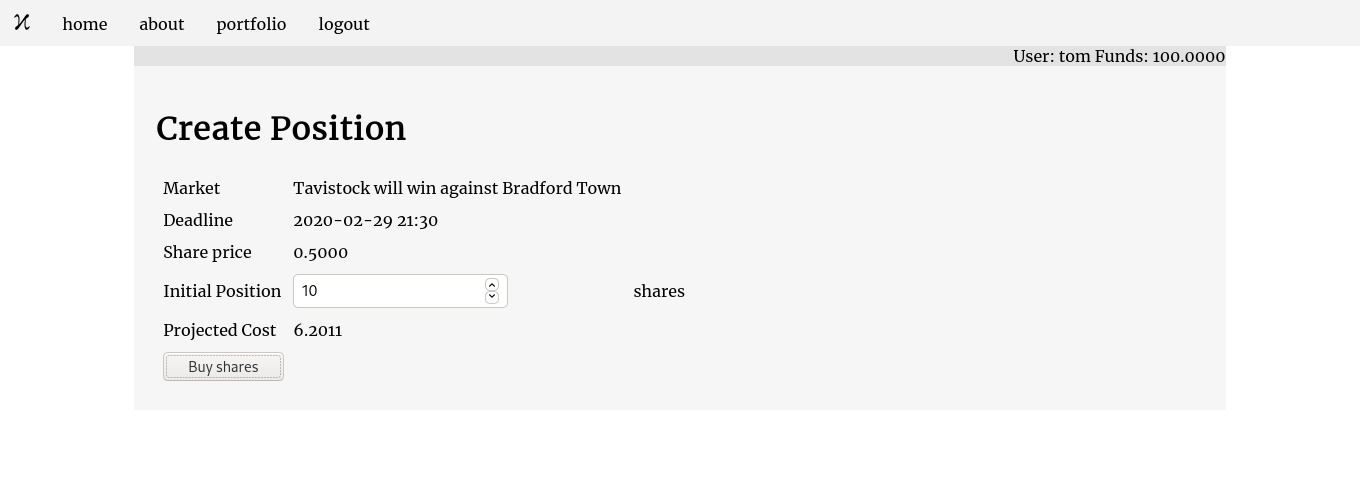
\includegraphics[width=\textwidth]{market-creation}
	\caption{The interface for creating a new market}
	\label{fig:marketCreation}
\end{figure}

\begin{figure}[h]
	\centering
	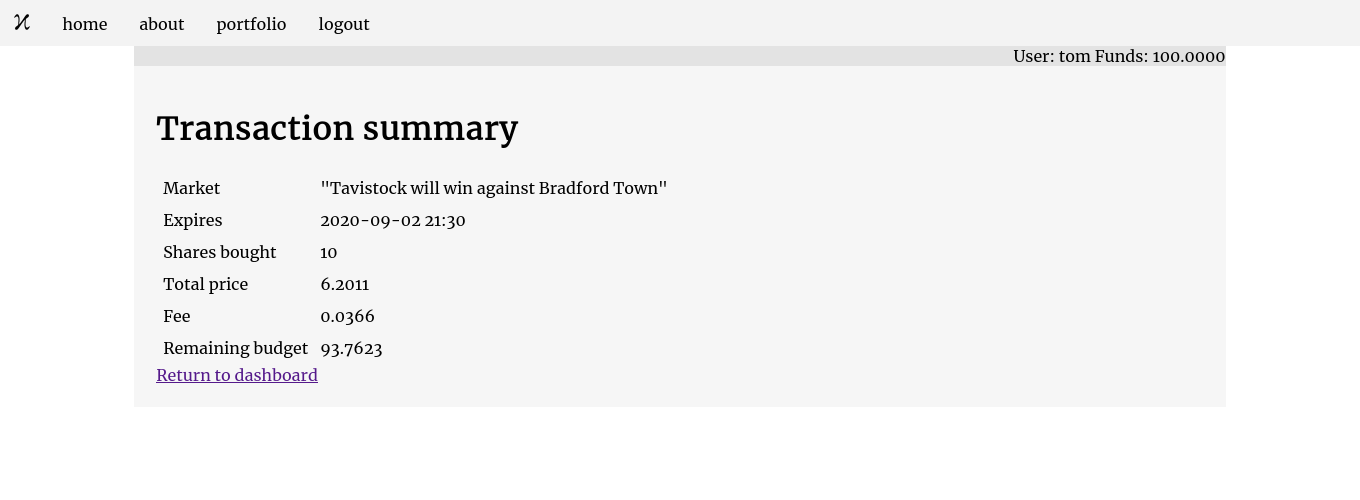
\includegraphics[width=\textwidth]{transaction-summary}
	\caption{Users are presented with a transaction summary upon creating a new
	market}
	\label{fig:transactionSummary}
\end{figure}

Fees are only charged on transactions where an agent increases their risk: this
means they are buying or selling a greater number of shares than their current
position. For example, a user owning ten shares and selling five would incur no
extra cost since they are liquidating a position they have already invested in,
while selling more than ten or buying additional shares would incur an
additional cost. The fee serves a secondary purpose in bounding the price of
the security away from \$0 and \$1, as a potential trader would be spending
more than \$1 or less than \$0 to buy or sell the shares. For example, even if
an agent were to buy an infinitesimal number of shares, meaning their
transaction cost would be given by the share price function $p$, if the share
price was \$0.99 and the transaction fee was set to 5\%, they would be required
to pay $\$0.99 \cdot 1.05 = 1.0395$, greater than the maximum possible payout.
This allows us to bound the total number of securities that will exist for a
given market, and hence its maximum payout.  In our market we implement a fixed
trading fee of 5\% on all risk transactions.

Obviously, we need to take into account a trader's budget when they are looking
to make a transaction and if they cannot afford one, deny them the trade. This
is simple for buy transactions, where the cost must not exceed their budget.
For a short sell, we need to ensure that the user will be able to cover the
expense of buying back the shares in the worst case -- that is, the event
occurs and they are required to buy back their position at \$1 per share. Hence
the function, \code{sufficient-funds?}, ensures a user can only go short on a
security if their budget plus the amount they are paid for shorting is larger
than the size of their short position.

\begin{figure}[h]
	\centering
	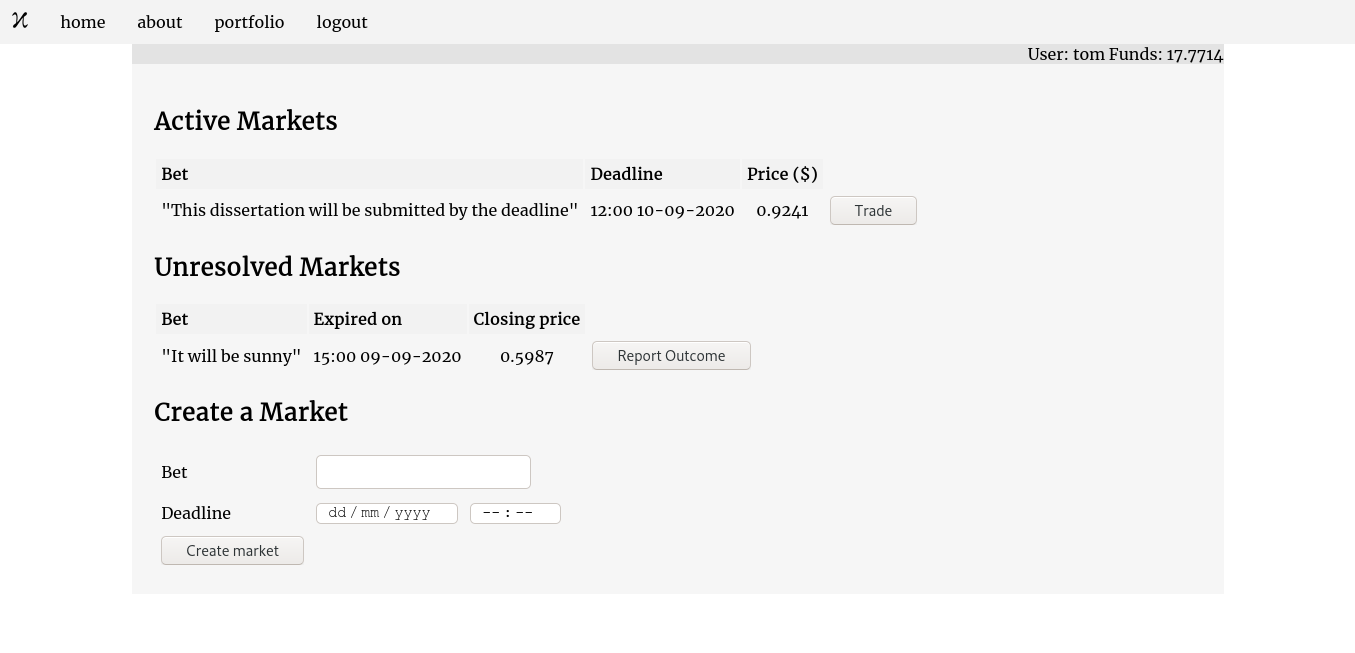
\includegraphics[width=\textwidth]{trade}
	\caption{Users can trade in active markets or report on those that have
	expired}
	\label{fig:trade}
\end{figure}

\subsection{Arbitration}

\label{sec:arbitration}

\subsubsection{Computing signal reliability}

The arbitration stage is where we resolve market outcomes using arbiter reports
and pay out winnings to, or demand payment from, stakeholders in the security.
Since the mechanism incentivises arbiters to act truthfully even if an arbiter
themselves holds a stake in the market, we decide to let anyone opt in to
reporting on the outcome. Once a market's deadline has passed the security will
be listed as an expired market and the user is presented with the option to act
as an arbiter, as in Figure~\ref{fig:trade} under ``Unresolved Markets''. After
doing so, they may then input their observed signal, or indeed a lie, as
Figure~\ref{fig:reportOutcome} shows. Once the required number of reports have
been collected, we move onto rewarding arbiters for submitting reports and
computing the final outcome of the market.

\begin{figure}[h]
	\centering
	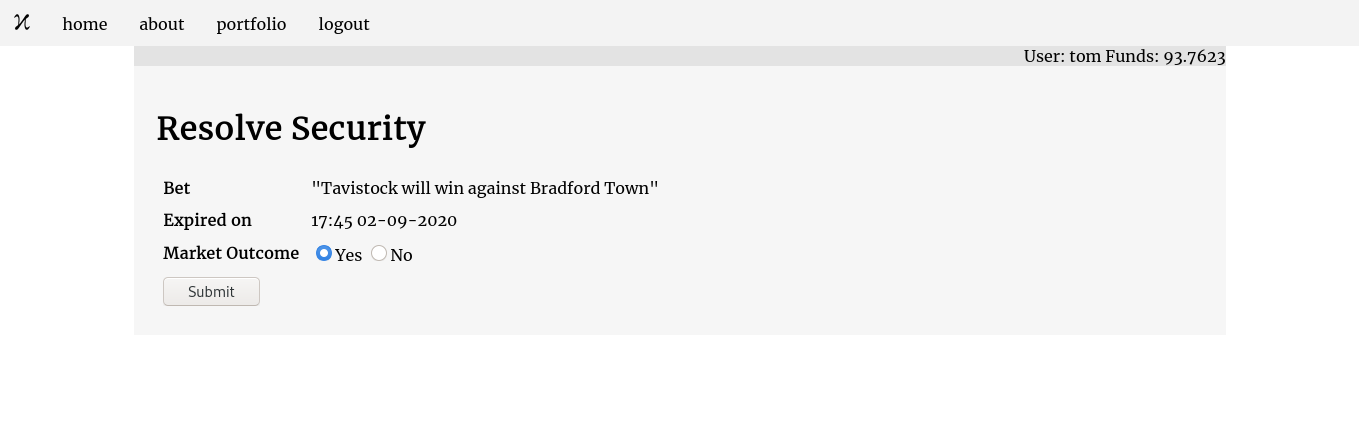
\includegraphics[width=\textwidth]{report-outcome}
	\caption{The interface by which arbiters report market outcomes}
	\label{fig:reportOutcome}
\end{figure}

%\begin{figure}[h]
%	\centering
%	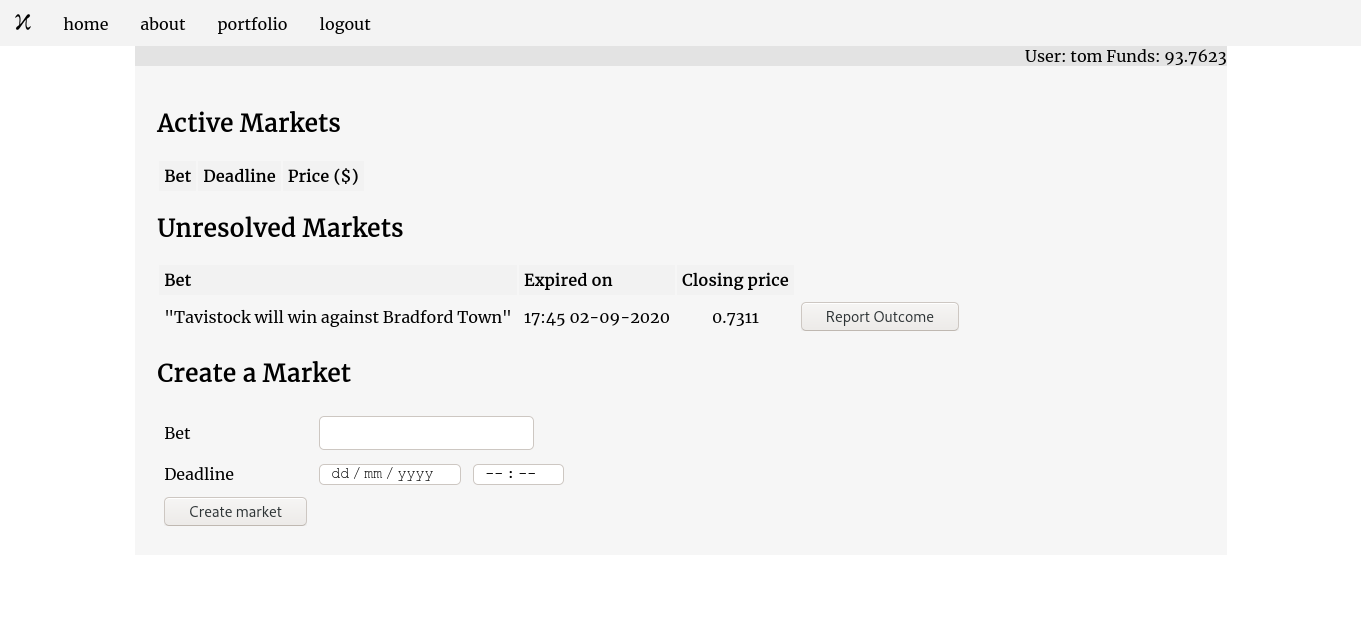
\includegraphics[width=\textwidth]{expired-market}
%	\caption{Users may opt in to report on market outcomes}
%	\label{fig:expiredMarket}
%\end{figure}

Arbiters are rewarded by being paid a certain amount of money only if their
report agrees with that of another randomly chosen arbiter. The reward is
determined by the 1/prior-with-midpoint mechanism, where instead of using the
common prior probability $\mu$ we use the update probabilities $\mu_1$ and
$\mu_0$. Recall that these are the probability that, given that arbiter $i$
receives a positive signal, so too does another randomly chosen arbiter $j$,
and the probability that, given that $i$ receives a negative signal, another
randomly chosen arbiter $j$ receives a positive signal. Since we cannot assume
arbiters to act truthfully, this is more complicated than simply counting the
types of reports received. Instead, we use information about signal error rates
$\Pr[x_i=1|X=1]$ and $\Pr[x_i=1|X=0]$ based on past market outcomes and past
reporting behaviour for each arbiter $i$. This is a fairly involved process:
first we gather all securities that have been reported on in the past by $i$
and whose outcome has been determined; we then iterate through each one of
these returned securities and determine the report that $i$ submitted as well
as its outcome, and push this into a list of results. At the end of this stage
we have a list \code{((security report outcome) ...)} that describes the
arbiter's report and the market's true (peer-determined) outcome for each
security for which they have acted as an arbiter. The code implementing this is
shown in Listing~\ref{lst:reportingHistory}.

\begin{lstlisting}[float,
	label={lst:reportingHistory},
	caption={Gathering a user's reporting history}]
(defun get-securities-reported-by-user (user)
  (with-open-database
    (select-dao 'security (inner-join 'user-security
                                      :on (:= :security.id
                                              :user-security.security-id))
                (where (:and (:= :user-security.user-id (user-id user))
                             (:not-null :security.outcome)
                             (:not-null :user-security.report))))))

(defun get-reporting-history (user)
  (let ((securities (get-securities-reported-by-user user))
        security-reports)
	(dolist (security securities)
	  (with-open-database
	    (let ((report (user-security-report
	                    (find-dao 'user-security
	                              :user user
	                              :security security)))
              (outcome (security-outcome security)))
	      (if outcome
            (push (list security report outcome) security-reports)))))
	security-reports))
\end{lstlisting}

We then use this history to compute the probability that, assuming the arbiter
has always acted truthfully, their signal has been correct in telling them the
true outcome of the event. We refer to these probabilities, $\Pr[x_i=1|X=1]$
and $\Pr[x_i=1|X=0]$, as a arbiter $i$'s positive and negative signal beliefs
as a remnant of a previous implementation. Listing~\ref{lst:positiveBelief}
shows how we calculate an arbiter's positive belief, with a similar method
applying for computing the negative belief: for the arbiter's history
restricted to the securities whose outcome was reported as positive by the
majority of arbiters, we count the number of times this arbiter also reported a
positive outcome, thus giving us the arbiter's signal error probability given
we know the outcome is (more likely to have been) positive. If there have been
no positive outcomes, then we assume the arbiter has a perfect signal.
Calculating the negative signal belief is done in a similar manner: first we
collect items of the arbiter's reporting history where the security was mostly
reported as a negative outcome, then we count the number of times this arbiter
submitted a positive report. Again we assume in the lack of markets with
negative outcomes that the arbiter has a perfect signal. We repeat this to
compute the positive and negative signal beliefs for each arbiter.

\begin{lstlisting}[float,
	label={lst:positiveBelief},
	caption={Computing an arbiter's positive signal belief given
	their reporting history}]
(defun calculate-positive-belief (reporting-history)
  ;; first only get the reports where the outcome was positive
  (let ((positive-outcomes (remove-if-not #'(lambda (x) (>= 0.5 (third x)))
                                          reporting-history))
        positive-reports)

    ;; now count the number of times the user reported a positive outcome
    (setf positive-reports (count T (mapcar #'(lambda (x) (equal 1 (second x)))
                                            positive-outcomes)))
    (if positive-outcomes
      (/ positive-reports (length positive-outcomes))
      1)))
\end{lstlisting}

We use this information about the reliability of each arbiter's signal, along
with the prior probability $\mu$ that the event had a positive outcome, to
compute the update probabilities $\mu_1$ and $\mu_0$, used in the
1/prior-with-midpoint mechanism. We first compute the update
probabilities $\mu_1^i$ for each arbiter $i$, using a randomly chosen peer
arbiter $j$, as follows:
%
\begin{equation}
	\label{eq:updateProbabilities}
	\begin{aligned}
		\mu_1^i & = \Pr[x_j=1|x_i=1] \\
		& = \Pr[x_j=1|X=0] \cdot \Pr[X=0|x_i=1] + \Pr[x_j=1|X=1] \cdot
		\Pr[X=1|x_i=1]
	\end{aligned}
\end{equation}
%
We use the same approach to compute $\mu_0^i$ for each $i$. The final values of
$\mu_1$ and $\mu_0$ are then calculated by taking the minimum and maximum
across all $\mu_1^i$ and $\mu_0^i$, respectively. Thus we have common update
probabilities across all agents.

\subsubsection{Rewarding the arbiters}

We may now pair arbiters randomly to pay them via the 1/prior-with-midpoint
mechanism. We first retrieve two lists from the database: the first is the list
of all arbiter reports and is of the form \code{arbiter-reports = ((arbiter
report) ...)}; the second is a list of all arbiter signal beliefs and is of the
form \code{arbiter-beliefs = ((arbiter positive-belief negative-belief) ...)}.
Since we will be pairing arbiters randomly and still need efficient access to
these values, we then create two hash tables associating an arbiter to their
report and their beliefs, giving us \code{report[i] = report} and
\code{beliefs[i] = (positive-belief negative-belief)} for each $i$. The
market's outcome is simply set to the proportion of arbiters that reported a
positive outcome. At this point we pay out the appropriate winnings to
stakeholders, paying out money to those who hold shares and demanding money
from those who have gone short. Now that the market's outcome has been
determined it will no longer be listed as an unresolved market on the user's
dashboard.

\begin{lstlisting}[float,
	label={lst:marketOutcome},
	caption={Computing the market outcome}]
(let ((reports (mapcar #'second arbiter-reports)))
  ;; the payoff of each share held is the fraction of arbiters reporting 1
  (setf outcome (float (/ (count 1 reports) (length reports)))))
\end{lstlisting}

We next compute the random pairing of arbiters. Lisp has no function to shuffle
a list, so we implement the Fisher-Yates
algorithm~\cite[pg.~26-27]{FisherYates1938} ourselves as the \code{shuffle}
function in Listing~\ref{lst:randomPairing}. The random pairing is then formed
by walking through the shuffled list and collecting adjacent elements as pairs.

\begin{lstlisting}[float,
	label={lst:randomPairing},
	caption={Assigning arbiters to peers randomly}]
(defun shuffle (lst)
  " shuffle LST randomly (without modifying it) "
  (let ((lst (copy-list lst)))
    (loop for i from (length lst) downto 2 do
          (rotatef (elt lst (random i))
                   (elt lst (1- i))))
    lst))

(defun random-pairing (lst)
  " randomly pair items from LST together if length(lst) is even "
  (if (evenp (length lst))
    (loop for (a b) on (shuffle lst) by #'cddr while b
          collect (list a b))))
\end{lstlisting}

For each set of paired arbiters we then retrieve their reports and signal
beliefs from the hash tables and compute, for each arbiter $i$ in the pair, the
values of $\mu_1^i$ and $\mu_0^i$ according to
equation~\eqref{eq:updateProbabilities}, where the randomly chosen $j$ is
simply the partner with whom they have been paired. We push these values to a
list so we may then compute the minimum value of $\mu_1^i$ and maximum value of
$\mu_0^i$ across all arbiters. Finally, to compute the smallest $k$ to satisfy
inequality~\eqref{eq:kBoundN} we set $k = \max_i 2|n_i|/m\delta$, and use this
to pay arbiters according to equation~\eqref{eq:oneOverPrior}.

\subsection{Server}

\label{sec:server}

The code from each of the separate areas of the market is then drawn together
in the file \code{server.lisp}, in which we set up the web server, define the
webpages, and call the functions from the different interfaces we provide.

We use Hunchentoot to host the web server. At startup this involves creating an
instance of a Hunchentoot \code{easy-acceptor}, which opens up a port of our
choosing to accept requests. Doing so also initialises the dispatch table,
which is a list containing the functions to execute when the corresponding
webpage is loaded. We can specify webpages to the dispatch table by using
Hunchentoot's \code{create-prefix-dispatcher} function: this simply takes a URL
and the function to execute when that URL is loaded. Again the opportunity to
use Lisp's macro system arises: the code in Listing~\ref{lst:defineURL} shows a
macro that defines a function and a URL of the same name, creates a dispatcher
for them and pushes it to the dispatch table. This again not only saves
rewriting repetitive code but also keeps the codebase clear -- for example, the
URL \code{/index} is served by a function called \code{index}. Now each time we
wish to define a new webpage we need only to call \code{define-url-fn} followed
by the name of the page and the code to execute.

\begin{lstlisting}[float,
	label={lst:defineURL},
	caption={Macroising URL functions}]
(defmacro define-url-fn ((name) &body body)
  " creates handler NAME and pushes it to *DISPATCH-TABLE* "
  `(progn
     ;; define the handler
     (defun ,name ()
       ,@body)

     ;; add the handler to the dispatch table
     (push (create-prefix-dispatcher
             ,(format NIL "/~(~A~)" name) ',name)
           *dispatch-table*)))
\end{lstlisting}

We use CL-WHO to define the content of the webpages, which translates Lisp
statements into strings of HTML. In order to achieve a consistent style while
avoiding code duplication we define a macro describing a ``standard page'', an
abridged version of which is given in Listing~\ref{lst:standardPage}. This
allows us to concisely define webpages with a similar look and feel, and only
requires us to specify the content that makes the page unique via the
\code{body} parameter.

\begin{lstlisting}[float,
	label={lst:standardPage},
	caption={Macroising webpage definitions}]
(defmacro standard-page ((&key title) &body body)
  " template for a standard webpage "
  `(with-html-output-to-string
     (*standard-output* NIL :prologue T :indent T)
     (:html :xml\:lang "en"
            :lang "en
            (:head (:title title)
                   (:link :href "/style.css" :type "text/css" :rel "stylesheet")
                   ;; rest of preamble ... )
            (:body
              (:ul :id "navbar"
                   (:li ... ))
              (:div :class "container"
                    ...
                    (:div :class "content"
                          ,@body))))))
\end{lstlisting}

Hunchentoot also automatically provides session handling -- this is obviously
important for allowing multiple users to be logged on at the same time and
presenting the appropriate information to them. All we need to do is define the
symbol \code{session-user} in the data structure for session handling, then
when a user logs in we set this value to the matching user retrieved from the
database with \code{(session-value 'session-user)}. This allows us to display
consistent user information across different webpages within the same session,
such as the user's budget or their portfolio of securities. Finally, users
mostly interact with the market through forms: Hunchentoot provides the
\code{get-parameter}, \code{post-parameter}, and \code{parameter} functions to
retrieve the values from these forms and send them to and from the different
webpages.

% session handling
% sending data e.g. (parameter ...)

\subsection{User Experience}

\label{sec:user-experience}

In Sections~\ref{sec:database}, \ref{sec:trading}, \ref{sec:arbitration}, and
\ref{sec:server} we have detailed the manner in which we achieve the goals laid
out in Section~\ref{enm:goals} which implement the core features of any
prediction market, as well as the behaviour that makes the peer prediction
mechanism of Freeman et al.\ unique. In this section we shall detail how we
make our prediction market more user-friendly and intuitive to use.

The most important aspect behind making the web application responsive is the
integration of asynchronous server communications so that we can display
up-to-date information to the user without a page refresh, as well as trigger
markets to close trading at the correct time. For this we use the Quicklisp
libraries Parenscript coupled with Smackjack to translate Lisp code to
JavaScript and allow us to communicate asynchronously with the server. We first
use Parenscript for form validation on the client-side, and in particular to
ensure that all required form fields are completed without needing to send the
entire form to the server, only for it to potentially be incomplete.
Parenscript provides the function \code{ps-inline}, which allows us to insert
Lisp code, that will be converted to a valid JavaScript program, within the
CL-WHO defined pages. We can therefore validate forms before being sent to the
server with \code{(form :action "create-market" :method :POST :onsubmit
(ps-inline ...))}. We implement form validation using a macro:
Listing~\ref{lst:nonEmptyMacro} shows the three functions we define to
dynamically check for completed fields. The function \code{make-nonempty-check}
simply writes Lisp code that, by the time it is called within \code{ps-inline}
will expand to the JavaScript statement \code{field.value == 0}. The function
\code{make-nonempty-list} allows us to simply specify a list of fields that we
require to be non-empty and have it generate a collection of non-empty checks.
Finally, the macro \code{nonempty-fields} calls the previous function and
splices it from a list to successive arguments to the \code{or} function. This
is all wrapped within a call to \code{ps-inline}, yielding something similar
to:

\begin{lstlisting}[
	label={},
	caption={},
	frame=none]
if (a.value == "" || b.value == "" || ... ) {
    alert("Please fill in all required fields");
}
\end{lstlisting}

\begin{lstlisting}[float,
	label={lst:nonEmptyMacro},
	caption={Macro for ensuring all required fields are complete}]
(defun make-nonempty-check (field)
  `(equal (getprop ,field 'value) ""))

(defun make-nonempty-list (fields)
  (loop while fields
        collecting (make-nonempty-check (pop fields))))

(defmacro nonempty-fields (msg &rest fields)
  `(ps-inline
     (when (or ,@(make-nonempty-list fields))
       (if (equal ,msg "")
         (alert "Please fill in all required fields")
         (alert ,msg))
       (return false))))
\end{lstlisting}

We use the Smackjack library in conjunction with Parenscript to implement AJAX.
Similarly to how we defined the webpage functions that execute when loading a
specific URL in Section~\ref{sec:server}, we must also push our various AJAX
functions to the dispatch table: Hunchentoot provides a special data structure,
similar to the \code{easy-acceptor}, that handles all asynchronous calls in the
form of the \code{ajax-processor}. We then create an AJAX dispatcher from this
and push it to the dispatch table as before: 

\begin{lstlisting}[
	label={},
	caption={},
	frame=none]
(push (create-ajax-dispatcher *ajax-processor*) *dispatch-table*)
\end{lstlisting}

We define all of our AJAX functions using the Smackjack macro
\code{defun-ajax}. This allows us to write functions in Lisp which perform some
computation on the server side and send a response back to the client
asynchronously. These function definitions are the same as any other in Lisp,
with additional information to specify the AJAX processor associated with it,
the method by which the data will be sent to the client, and the format that
the client should expect it in. We use only one processor,
\code{*ajax-processor*}, which is initialised when the server starts, and we
send all data via an HTTP POST request as a JSON string.

One manner in which we use this asynchronous communication is to quote a
projected cost of a transaction to a user looking to trade. Since we require
the number of shares a trader is looking to buy or sell in order to quote
$C_b(q')-C_b(q)$, and we wish to do this without a page refresh, we implement
the cost function as an AJAX function that takes the user's desired quantity of
shares and the current total number of shares in the security to quote the
cost. The interface we present to the user restricts them to entering positive
quantities only and checking a button to specify whether to buy or sell (since
entering a negative number to sell could be confusing), hence we also need the
value of this radio button to compute the transaction cost. This function is
given in Listing~\ref{lst:ajaxTransactionCost}. The function is now defined
within Smackjack's namespace: next we need to define the function that calls it
asynchronously in JavaScript.

\begin{lstlisting}[float,
	label={lst:ajaxTransactionCost},
	caption={Defining an AJAX function for computing transaction cost using
	Smackjack}]
(defun-ajax ajax-transaction-cost-quantity (quantity q buying-p)
			(*ajax-processor* :method :POST :callback-data :json)

			(if (stringp quantity) (setf quantity (parse-integer quantity)))
			(if (stringp q) (setf q (parse-integer q)))
			(let ((q* (if buying-p
						(+ q quantity)
						(- q quantity))))
			(format NIL 
					"{\"newShares\" : ~D, \"oldShares\" : ~D, \"cost\" : ~4\$}"
					q*
					q
					(msr:transaction-cost q* q))))
\end{lstlisting}

The JavaScript functions that call the AJAX functions need to be defined within
the usual \code{script} tags, for which we simply wrap the appropriate Lisp
code in the \code{(:script ...)} macro provided by Parenscript. For retrieving
the transaction cost of a given trade, we define the function
\code{ajax-transaction-cost-trade} as in
Listing~\ref{lst:javascriptTransactionCost}. This function is responsible for
getting the quantity of shares the user has input, the current outstanding
quantity of shares, and which radio button has been checked to specify whether
they are buying or selling. This is achieved by the Parenscript macro
\code{chain}, which chains the list of arguments following it into a list of
function calls and attribute retrievals as required. Note that the two radio
buttons specifying whether to buy or sell must necessarily have the same
\code{id} and \code{name} field within the form, hence we cannot simply call
\code{get-element-by-id} to retrieve the value. Instead, we call
\code{get-element-by-names} to return both, then iterate through them to verify
which one was checked. We then call the AJAX function we defined earlier from
Smackjack, \code{ajax-transaction-cost-quantity}, to compute the transaction
cost. This then triggers the callback function \code{display-projected-cost},
which actually updates the value in the appropriate table cell asynchronously.
Listing~\ref{lst:javascriptTransactionCost} reflects the rest of this process.

\begin{figure}[htp]
	\subfloat[]{%
		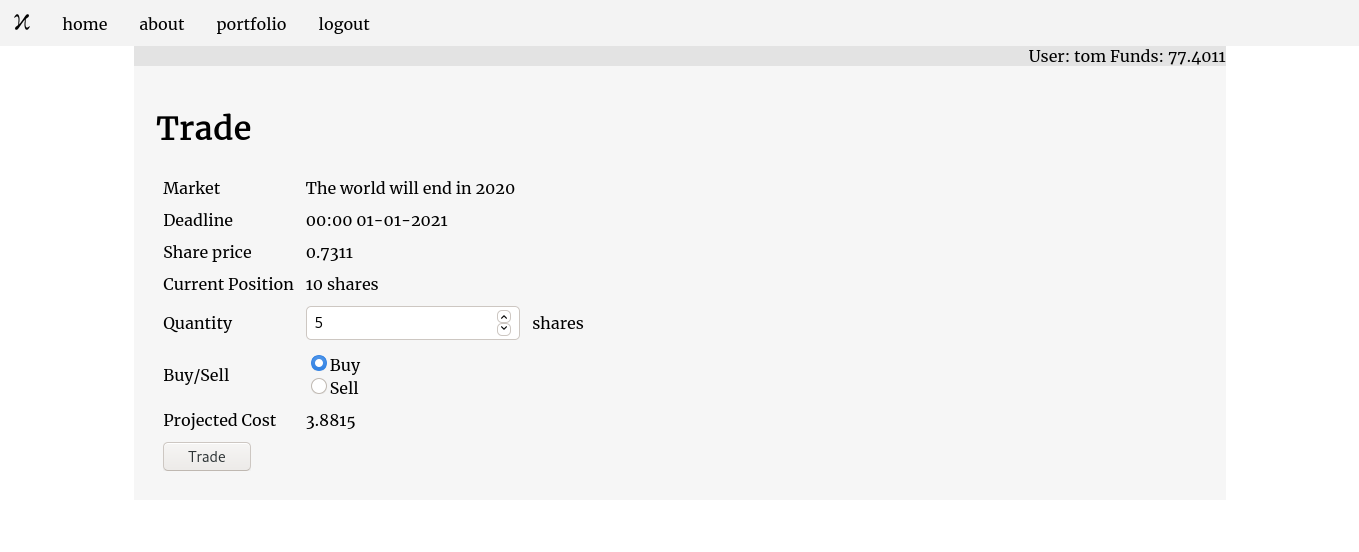
\includegraphics[width=\textwidth]{ajax-price-1}%
	}

	\subfloat[]{%
		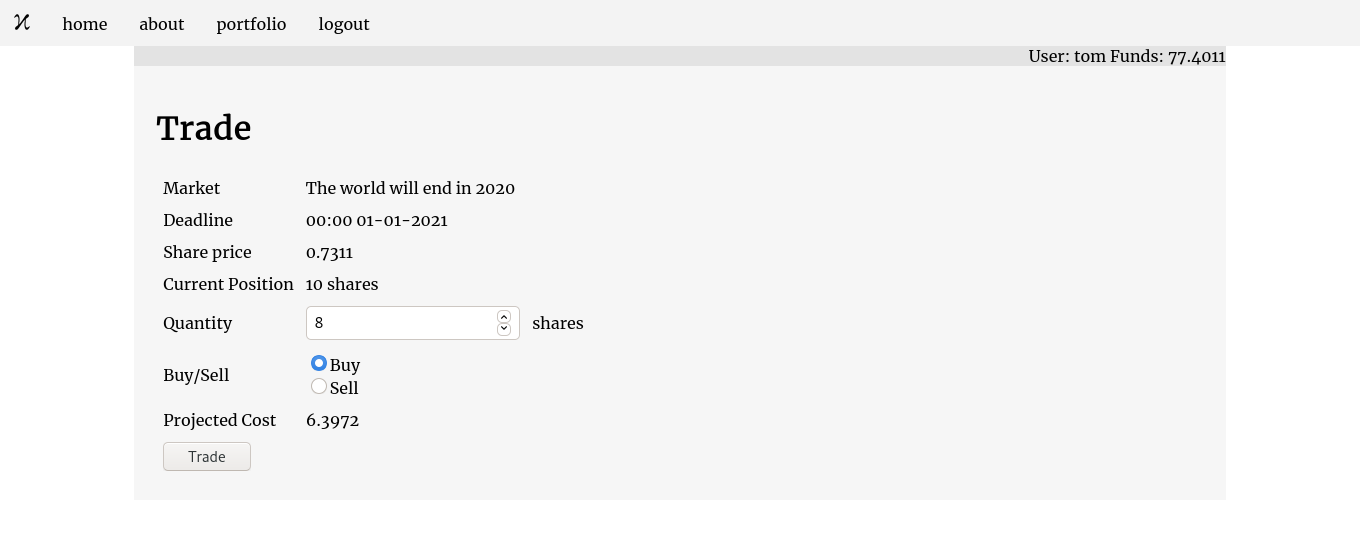
\includegraphics[clip,width=\textwidth]{ajax-price-2}%
	}
	\caption{Updating transaction costs asynchronously}
\end{figure}

\begin{lstlisting}[float,
	label={lst:javascriptTransactionCost},
	caption={Calling the AJAX function asynchronously}]
(ps
  (defun ajax-transaction-cost-trade ()
	" calculate transaction cost when trading in market "
	(let ((quantity (chain document (get-element-by-id :quantity) value))
		  (q (chain document (get-element-by-id :old-shares) value))
		  (radios (chain document (get-elements-by-name "buying")))
		  checked
		  buying-p)

	  ;; find which radio button is checked
	  (loop for option in radios do
			(if (@ option checked)
			  (setf checked (@ option value))))

	  ;; checked is equal to 1 if "buy" is selected
	  (setf buying-p (equal checked 1))

	  (chain smackjack (ajax-transaction-cost-quantity
						 quantity
						 q
						 buying-p
						 display-projected-cost)))))
\end{lstlisting}

Finally, we use AJAX to automatically close trading when a market's deadline
has passed. We first define a Smackjack function that retrieves the most
imminently expiring security, then compute the difference in seconds between
the current time and its deadline. A JSON object is then returned containing
this value, which we use to set a timer for the page to reload. We next define
the Javsacript function \code{set-timer} which takes this JSON object and sets
the page to reload after this interval. This process is given in
Listing~\ref{lst:setTimer}. This prevents user from trading shares after
potentially knowing the outcome, and instead reloads the page and lists the
market under ``Unresolved Markets'' and no longer active (see
Figure~\ref{fig:trade}).

\begin{lstlisting}[float,
	label={lst:setTimer},
	caption={Triggering the close of trading automatically}]
(defun-ajax ajax-set-timer ()
			(*ajax-processor* :method :POST :callback-data :json)

			(let ((next-expiring (db:get-next-expiring-security
								   (local-time:now)))
				  timer)
			  (unless (equal next-expiring NIL)
				(setf timer (local-time:timestamp-difference
							  (db:security-deadline next-expiring)
							  (local-time:now)))
			  (format NIL "{ \"security\" : ~S, \"seconds\" : ~D }"
					  (db:security-bet next-expiring)
					  (ceiling timer)))))

;; within a (:script) tag elsewhere ...
(ps
  (defun set-timer ()
	(chain smackjack
		   (ajax-set-timer #'(lambda (response)
							   (set-timeout (lambda ()
											  (chain location (reload)))
									 		(* (@ response seconds) 1000)))))))
\end{lstlisting}

\section{Project Management}

\label{sec:projectManagement}

\subsection{Methodology}

The project has been developed incrementally, with a focus on integrating new
functionality completely before progressing to new features. This approach is
well-suited to this project's design: since it consists of five separate areas
which are drawn together at the end, it is possible to focus on implementing a
feature within one area without it affecting the rest. As a result, testing has
been performed throughout and ensures that a newer version of the project is
never worse than its predecessor. Using Git and Github has been helpful in this
regard, providing cloud storage and the ability to roll back to previous
versions of the project if the current one is broken by a new feature.

\begin{figure}[h]
	\centering
	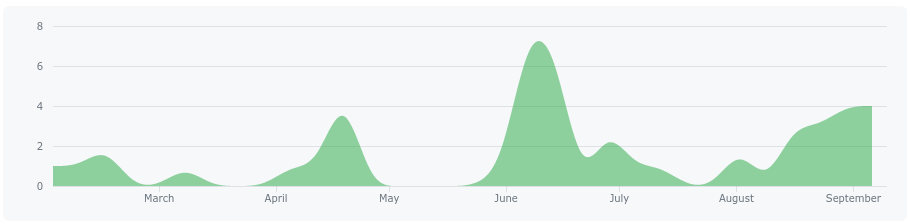
\includegraphics[width=\textwidth]{commits}
	\caption{Commits to Github}
	\label{fig:commits}
\end{figure}

Meetings have been taken with this project's supervisor, Professor Matthias
Englert, to track progress. These were more regular towards the beginning of
the project, though as it began to take shape the consistency of these meetings
declined. As we will discuss in the following section, this is due in part to
the exam period, during which most focus was diverted towards revision, however
the original frequency was never picked up after this time as was initially
planned. Moreover, it bears mentioning that the current situation regarding the
coronavirus pandemic may also have had a part to play in the frequency of these
meetings. Regardless, the author feels more initiative should have been taken
on his end to ensure their consistency, even with the move online.

\subsection{Scheduling}

There have been few major issues with regard to the scheduling of this project,
although it undergone a slight change from the timetable in its original
conception, which was meant to be an implementation of a combinatorial
prediction market similar to \emph{Predictalot}. Figure~\ref{fig:old-timetable}
shows the schedule as it was planned at the time of our presentation on the
project, which was when it was still in its early stages of development. In
Figure~\ref{fig:new-timetable} we detail the order in which tasks were actually
carried out.

\begin{figure}[h]
	\centering
	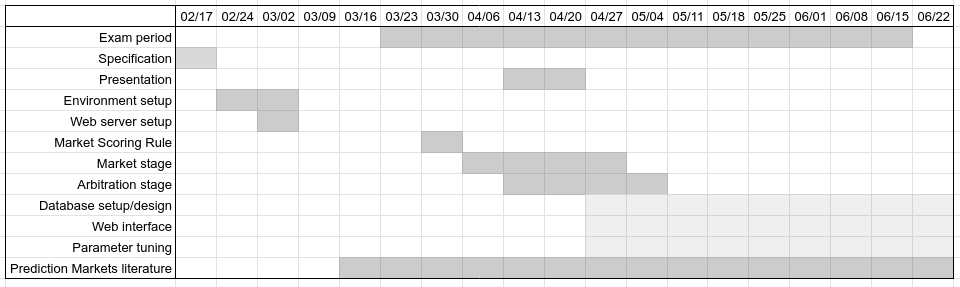
\includegraphics[width=\textwidth]{old-timetable}
	\caption{The project's timetable as it was initially planned}
	\label{fig:old-timetable}
\end{figure}

An initial prototype of the prediction market had been written in time for the
presentation and at its core our current iteration is very similar to this
early version with respect to the datatypes we define and the processes of
trading and arbitration. However, it was entirely text-based and had no
capacity for persistent storage, meaning it was unusable in a practical
setting. At any rate its purpose was to showcase the mechanism in action and
this is, at its core, very simple. 

Work after this point was focused on translating this terminal-based
implementation to operate on a barebones web server, with the first steps to
achieve persistent storage via interaction with a database. Since Mito's
\code{deftable} macro is functionally very similar to that of Common Lisp's
\code{defstruct}, this conversion was relatively straightforward. Similarly,
the code to set up and begin defining webpages in our implementation is simple
and hence took little time. In the case of both the web server and the
database, a significantly larger portion of time was spent deciding how to
integrate features as they were developed into the system as a whole. As we try
to keep our implementation modular there is the implicit requirement to not
only get a feature working in isolation, but to then integrate it into the rest
of the system successfully. This involved constantly updating the web and
database interfaces, and is reflected in Figure~\ref{fig:new-timetable}, which
shows much more overlap between tasks.  Some issues were encountered trying to
implement asynchronous communication with the server via Parenscript and
Smackjack, and much time was spent getting this working. This highlights one of
the drawbacks behind using both libraries: while they are somewhat
well-documented with online reference manuals, it seems they are not widely
used and hence have few practical examples from which to learn.

Worthy of note is the two-week delay from the original deadline for the interim
report, arising from the university-wide implementation of a two-week extension
to all assessed work. We decided to take advantage of this by spending an extra
two weeks to implement the arbitration stage to a greater degree of completion,
in order to have more material for discussion in the interim report. This in
part stems from the fact that we had made less progress during and after the
exam period as expected. This did not affect the overall progress of the
project, however, since the two weeks worth of progress made during this time
was simply borrowed from what would have been achieved in the two weeks after
the original deadline. 

\begin{figure}[h]
	\centering
	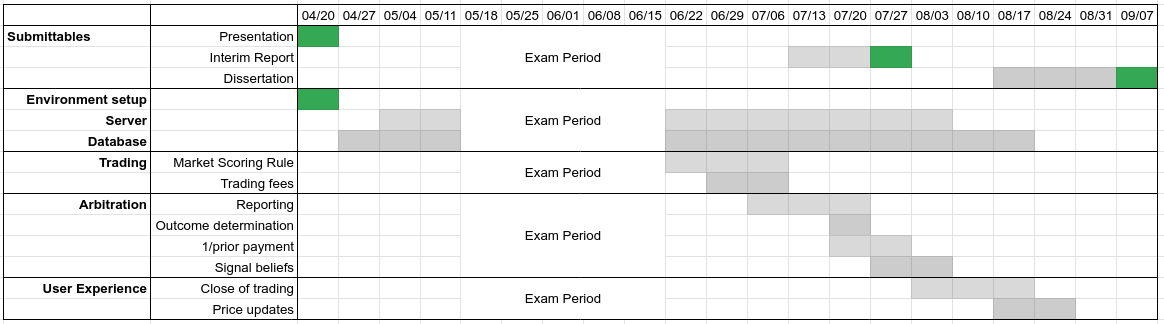
\includegraphics[width=\textwidth]{new-timetable}
	\caption{The realised schedule}
	\label{fig:new-timetable}
\end{figure}

\subsection{Ethics}

There is little ethical consideration required for the development of this
project. All development and testing has been done independently, and all
resources used to implement the system are available freely. Testing has been
performed externally only to small extent, and even then only informally
through gathering opinions amongst colleagues. As we have discussed has been a
problem for existing prediction markets, there is one ethical issue that arises
from using real money in prediction markets and this is their potential to
inspire ``assassination markets'', where there is a real-life incentive to
change the outcome of the market through committing actions of dubious
character, such as assassinating the subject of a security speculating on the
time of their death. We avoid testing the strength of our users' moral fibre by
using fake money only, with no real-world value, meaning there is no incentive
to act in such a way as to compromise one's integrity for monetary gain.

\section{Evaluation}

\label{sec:evaluation}

In this section we shall begin by reflecting on some of the successes of the
project, followed by suggestions of improvements that could be made to our
implementation were we to have more time. We conclude with a reflection on the
project as a whole.

\subsection{Successes}

One obvious success of the project is that we have implemented the
decentralised prediction market that we originally intended based on the work
of Freeman et al. A key component of the market is that participants are
incentivised to act in the desired way through paying each user a specific
amount of money. This has required building a strong understanding of their
paper to ensure everything has been implemented correctly so that we may
achieve the theoretical guarantees that they outline.  We have also managed to
become more well-acquainted with the wider literature on prediction markets; a
key goal motivation before choosing a project had been to gain more exposure to
the field of algorithmic game theory, and in this regard the project has been a
personal success.

Translating the mechanism Freeman et al.\ from a theoretical setting into a
practical environment has required slightly modifying certain aspects of it to
make it functional in the real world, especially with respect to the
assumptions we can make. For example, the paper uses the following bound on the
number of securities to calculate the minimum payment required in the
arbitration stage to incentivise truth-telling:
%
\begin{equation}
	\label{eq:kBoundB}
	k \ge \frac{2 B (1+f)}{f m \delta}
\end{equation}
%
in which $B$ is the maximum amount of money that any single agent can spend in
the market. They use the above inequality instead of
inequality~\eqref{eq:kBoundN} as they view knowledge about an upper bound on
the number of securities that any single agent owns, $|n_i|$, as ``an
unsatisfying restriction''. However, since we are the prediction market, we
require knowledge about each agent's position in order to pay out winnings
appropriately by the time the event has taken place.  Hence we can use
inequality~\eqref{eq:kBoundN} to calculate the minimum value of $k$, giving a
more direct means of computing the parameter and a more exact bound.

Another modification we make is in our calculation of what we have referred to
as a user's ``positive signal belief'' and ``negative signal belief''. These
are so named because in an earlier version of the market, each time an arbiter
was asked to report on an event's outcome they would be asked for an estimation
of $\Pr[x_i=1|X=1]$, the probability that they receive a positive signal given
the true result is positive; and $\Pr[x_i=1|X=0]$, the probability that they
receive a positive signal given the event was truly negative. Freeman et al.\
assume knowledge of the news sources from which users gain their signals -- for
example, for some political event it is known that 10\% of the population
checks only liberal or left-leaning news sources, while 10\% check only
right-leaning sources. These signal probabilities therefore directly follow. In
practice this is completely unrealistic, since users may check a variety of
news sources at varying points on the political spectrum, so we cannot know
from where exactly which proportions of the population are getting their
information. Instead, we compute the signal beliefs using each arbiter's
reporting history and the true outcomes of the events they have reported on.
This gives us an idea of the signal each arbiter receives on average. However,
this value will not change from market to market, meaning we are less
well-equipped to deal with ambiguous wagers since an arbiter has no way to
signify to the system that the bet was indeed unclear or open to
interpretation. Having the value of $\delta$, the ``update strength'', vary
between markets allows the $k$ from equation~\eqref{eq:oneOverPrior} adjust
payments according to its perceived ambiguity. This issue is, however, somewhat
mitigated by the likelihood that most bets submitted on our market will be
unambiguous in nature.

One final variation that we make to the original mechanism is that we keep the
trading fee $f$ fixed. The reason for this is twofold: firstly, it relies on
$\delta$, which as we have just discussed does not vary for different markets
as it is always calculated from an arbiter's history for \emph{every} market.
If our value of $\delta$ is just an estimate, it can be argued there is little
sense in trying to set $f$ as precisely as possible. Secondly, we have not yet
been able to calculate $f$ dynamically in the allotted time. Its calculation
involves other variables and would likely require changes to various other
parts of the system, in particular the database, which could jeopardise the
system's current working state before submission. At any rate, this is
something we wish to implement in the future as, regardless of how much
$\delta$ changes, it guarantees that the mechanism generates enough revenue to
pay arbiters without requiring outside subsidisation. We currently have $f$ set
to 5\% as Freeman et al.\ show empirically that this relatively high fee can
subsidise ambiguous markets with low values of $\delta$ and high participation.
However, since it is not set dynamically, there is no way of knowing whether it
will be enough to cover arbitration costs -- only once we find ourselves paying
out more than we have will we know we have made a mistake. We can avert this
crisis by overestimating the value of $f$ required, which is the solution we
currently opt for, but this is certainly a less satisfying solution. Overall,
we consider our implementation a success as the tweaks we make to the mechanism
allow it to be realised in a practical setting that does not require
unrealistic assumptions to be made.

Finally, while not necessarily important from an academic perspective, we
consider the project a success for having been implemented in the Lisp
programming language, with which we had had no experience prior to starting the
project. It has at times rendered development more challenging and introduced
obstacles that would not have ordinarily been there -- for example, worrying
about whether a Parenscript and Smackjack statement would translate to the
correct JavaScript, as opposed to simply writing the correct JavaScript
straight away -- although the features of the language have also made it a more
rewarding experience. In addition to harnessing the power of macros, its
functional style along with its simple, consistent syntax has oftentimes
allowed for the code to be written in a clearer, more concise manner.

\subsection{Next steps}

\subsubsection{Additions}

There are numerous improvements we can make to our market, and while we have
implemented all necessary features of the paper on which we base the mechanism
itself, such additions would be significant in increasing the usability of our
system. These fall into two categories: those that add new functionality, and
those that improve on the existing codebase.

A key feature missing from the system currently is the ability to plot graphs
of a market's share price. This would greatly improve the usability of the
system and would be an effective analytical tool to visualise a security's
price movements over time. Since share price is a proxy for the community's
beliefs on the outcome of the corresponding event, this would be useful in
observing how public sentiment changes throughout a market's lifetime as a
result of the agents receiving new information. It appears there is plenty of
choice regarding libraries that would allow one to plot such graphs, such as
ADW-Charting and CGN, which are both available through Quicklisp.

One way to generalise the mechanism we have implemented would be to allow for
different types of events to be wagered on. Currently, users may only submit
events whose outcome is either a ``yes'' or a ``no'' -- this could be improved
upon by allowing for categorical markets, in which traders are offered to buy
or sell shares in more than two mutually exclusive outcomes. For example, a
market could be created on the bet, ``Which country will host the 2032 Olympic
Games'', with options to invest in Germany, Italy, the United States, and
Canada. There are two issues with this that prevented it from being explored
within the time-frame of this project. Firstly, a great deal of the analysis of
\cite{Freeman2017} relies on the assumption that traders are participating in a
binary market, hence much of the parameters would have to be derived again in
order to successfully translate the incentive-compatible mechanism to the
categorical setting. While this is feasible over a longer period, the idea came
too late to be possible in the remaining time. Secondly, the codebase would
need to be altered significantly to allow for this generalisation. It could be
beneficial, since binary markets are just subsets of categorical ones, however
the system would require a large rewrite to generate the HTML dynamically and
deal with the added complexity.

Finally, a longer term goal would be to apply the approaches of Kroer et
al.~\cite{Kroer2016} to our market to translate it to a combinatorial setting.
However, the extent to which this can be done appears to be very limited: a key
component of the mechanisms they analyse is that the securities are related in
some way, meaning a user's participation in one security can affect the odds of
another. The degree to which a new security is related to other existing
securities is controlled by the market creator, who for example sets the
initial price and specifies the constraints used in solving the integer
programs. This would be counter-productive in our setting since we rely on
users to create the markets themselves: either we allow users to control these
parameters, in which case we must incentivise them to act truthfully, or we
specify them ourselves, which may be inaccurate and negates the point of
implementing a decentralised market in the first place.

With more time, we would also look to implement more responsiveness from the 
system. This would include building on the JavaScript code already in place to
have prices constantly updating, so that users are informed of price changes as
they happen and they may execute trades at these up-to-date prices. Similarly,
countdowns for markets whose deadlines are imminent would be useful in not only
making the interface feel more alive but also in generating urgency and
encouraging user participation.

\subsubsection{Improvements}

Currently we allow any user to create a market for an event of their choosing.
We require that upon creating the market, they are only able to buy
shares. This is a natural restriction that means users only make markets for
events they believe will, more than likely, occur. However, there is nothing to
stop them from simply negating the statement and creating a market for this.
Although not a serious issue, this may lead to unnatural or unclear phrasing,
in which case it would simply be better to allow them to go short initially.
An issue related to this is that we do not verify the bets that users place,
and therefore there could be duplicate markets on the same event whose prices
do not match. Clearly buyers are encouraged to trade in the lower priced one,
and sellers the higher priced one, leading to a discrepancy in the forecasts we
make. We do not currently see a good solution to this problem.

An issue in our implementation is that of deciding when there are enough
reports. Instead of randomly selecting users to act as arbiters, which may
cause delays in determining the outcome of the market as we must wait for each
arbiter to report, we allow any user to act as an arbiter, hopefully increasing
the speed with which we can close markets. Thanks to how we set the parameter
$k$ in equation~\eqref{eq:oneOverPrior}, arbiters are incentivised to act
truthfully regardless of whether they hold a stake in the market. However, it
is undecided how the number of arbiters required should scale with the size of
the userbase: it is currently set to two for ease of testing, though it will
somehow need to increase with a growing community (up to a point). This in turn
allows for finer control over the payout per share.

Finally, there are several sources of avoidable inefficiency in our code.
Firstly, consider the fragments given in Listing~\ref{lst:reportingHistory}.
In order to get a user's reporting history we first retrieve all of the
securities reported on by the user from the \code{SECURITY} table, then we
iterate over these returned securities and retrieve the securities whose
outcome has been determined: this involves executing one query for each parent
record and another for each child record. This is known as the $N+1$ query
problem and is common among ORMs such as Mito. We can achieve equivalent
behaviour for a fraction of the queries using eager loading, which executes a
single query to retrieve each child record. Mito has a specific macro for this,
and given this pattern's prevalence in our codebase, would make for a useful
improvement. We use our \code{with-open-database} macro, given in
Listing~\ref{lst:databaseMacro}, to define many of the functions exposed by the
database interface. Problems of inefficiency could arise when calling numerous
of these functions sequentially, since a connection would be opened and closed
for each one. It would be more efficient to connect only once, execute all
transactions, and then disconnect. At present, we do not see a solution to this
that keeps the benefits of macroising the interactions with the database in the
first place.

\subsection{Closing Remarks}

Overall, this project has been successful and we have enjoyed building an
understanding of the literature surrounding prediction markets, as well as
gaining proficiency in Lisp. One criticism of the project is that it does not
necessarily offer something new, since we base our design on an existing
mechanism in order to achieve their guarantees. While we implement the peer
prediction market and make necessary adaptations to make it suitable for
real-world use, there are no novel results that arise from our work. The
alternative, of proving some new theoretical result, would of course have been
an unlikely task in the time frame, although the project could have perhaps
benefited from being more ambitious. At any rate, what we implement here can be
used as an effective tool to calculate forecasts on a wide array of bets and is
open to further extension to increase the potential for real-world use.

We will leave our prediction market running for as long as possible after
submission here: \url{https://1a091f61d58d.ngrok.io/index}. Many thanks go to
Matthias for supervising this project, in suggesting to look at prediction
markets, and for helpful advice throughout.


% Evaluation points
% - Ugly design pattern of `select-dao` then iterating with LISP (not SQL)
% - Not enough tutor meetings
% - Unrealistic to ask users to supply signal beliefs -- unlikely they know, but
% 	alternative is to have central person deciding on it and removing
% 	decentralisation
% - Too much processing code in server.lisp -- separate out into interfaces
% - Grace period? Time where no shares can be traded to prevent ambiguous
%   markets getting tanked by later investors
% TODO: eager loading in database

\bibliography{bibliography}

\begin{appendices}

\end{appendices}

\end{document}
